    \documentclass[12pt]{article}
     \usepackage{tikz}
    \usepackage{multirow}
    \usepackage{geometry}
    \geometry{a4paper, margin=1in}
    \usepackage{titlesec}
    \usepackage{lipsum} 
    \usepackage{tabularx}
    
    \usepackage{graphicx}
    \usepackage{float}
    \usepackage{amsmath}
    \usepackage{titlesec}
    \usepackage{hyperref}
    \usepackage{enumitem}
    \usepackage{tikz}
    \tikzstyle{block} = [rectangle, draw, fill=blue!15, 
    text width=10em, text centered, rounded corners, minimum height=3em]
    \tikzstyle{arrow} = [->, thick]
    
    \titleformat{\section}[block]{\filcenter\bfseries\Large}{\thesection.}{1em}{}
    
    
    % Set the subsection title format
    \titleformat{\subsection}
    {\normalfont\large\bfseries}{\thesubsection}{1em}{}
    
    \begin{document}
    
    \title{RA weekly Report}
    \author{Hariom Mewada\\
    24M2137}
    \maketitle
    
    \newpage
    \tableofcontents
    \newpage
    
    \section{Octobor 14, 2024 - Octobor 21, 2024}
    % \subsection{To Do List}
    % \begin{itemize}
    %     \item Understand the Matchfixer system.
    %     \item Setting up Matchfixer on local machine.
    %     \item Understand How SSO Works.
    %     \item Creating new branch to work on.
    %     \item Feature to change TA vacancies for course
    
    % \end{itemize}
    \subsection{Understood the intenton UI code}
        \begin{enumerate}
            \item understood various modules of the intentor app like how
            \textbf  {dashboard}, \textbf{Challenges} and \textbf{Daily usage limit} works
            .
            \item Understood  \textbf{ Count of locks and usage count Notification}, \textbf{Login},\textbf{alertlaunch} subsection of the App.
    
             % \item Understand  \textbf{Frictional Challenges}, \textbf{Strict vs cancellabel},\textbf{Personal Stories} , \textbf{Sharing performace with friend} subsection of the library.
            
            \item Went through code  to understand their working. 
        \end{enumerate}
        
    \subsection{Setting up Android Studio and Intentor on local machine}
        \begin{enumerate}
            \item Downloaded \textbf{JDK} ,\textbf{Android Studio},\textbf{Github}.
            \item  Cloned intentor repo and checkout to to \textbf{Master} branch to fetch latest code.
            \item Setup environment for packages installation and \textbf{JDK} for running Android Studio.
             \item Understood various terminology and concepts related to \textbf{Android Development}
        \end{enumerate}
    \subsection{Development of Digital Detox Library}
    \begin{enumerate}
        
    \item Started implementation of library with various usefull features like \textbf{Session}, \textbf{Scheduled Session} ,\textbf{Pause} ,\textbf{InterSessionGap}, \textbf{Challenges}
    which can further extend the functionality of intentor App very smoothly.
    \end{enumerate}
    \subsection{Future Goals}
    \begin{enumerate}
      
        \item \textbf{Add Customizable Challenge Types:} Expand the challenge types for users to include mental, physical, and cognitive tasks to further discourage excessive social media usage.
        \item \textbf{Enhance Challenge Verification:} Implement stronger challenge verification mechanisms, like integrating quizzes, puzzles, or tasks requiring user interaction (e.g., image or voice recognition).
        \item \textbf{Usage Insights \& Analytics:} Build a system to track app usage patterns and provide personalized feedback to users based on their activity levels, including metrics like total screen time, app usage frequency, and longest continuous sessions.
        \item \textbf{Notifications and Reminders:} Add features that remind users to complete challenges or display motivational messages when their usage time exceeds the set limit.
        \item \textbf{User Profiles and Data Syncing:} Store user preferences and challenge progress in a profile system that supports cloud syncing, so users can manage their data across devices.
    \end{enumerate}
     \subsubsection{Research and Testing}
     \begin{enumerate}
         \item \textbf{Behavioral Research:} Study behavioral trends around social media addiction to refine the library and create more effective mechanisms for user control.
         \item \textbf{Usability Testing:} Conduct usability studies with a group of users to gather feedback on  the overall user experience.
     \end{enumerate}
    
    \section{Plans for  RA work}
    \subsection{Analyze and Optimize Existing Features}
    \begin{itemize}
        \item \textbf{Review User Feedback}: Gather and analyze feedback from current users to identify pain points or missing features.
        \item \textbf{Bug Fixing and Optimization}: Identify and resolve existing bugs or performance issues to improve the user experience.
        \item \textbf{UI/UX Enhancements}: Update the interface to make it more user-friendly and visually appealing.
       \item \textbf{Explore similar product in market}: Explore and analyze feature offered by other similar applications in market
    \end{itemize}
    
    \subsection{Enhance Functionality}
    \begin{itemize}
        \item \textbf{Customizable Challenges}: Allow users to select preferred friction challenges or adjust their difficulty levels.
        \item \textbf{App Usage Analytics}: Implement a dashboard showing detailed usage statistics (e.g., time spent on apps, frequency of unlocking challenges).
        \item \textbf{Notification Scheduling}: Add a feature to schedule reminders or restrict app access during specific times.
    \end{itemize}
    
    \subsection{Strengthen App Monitoring}
    \begin{itemize}
        \item \textbf{Foreground App Detection}: Improve the accuracy of identifying apps in the foreground and detecting patterns.
        \item \textbf{Battery Optimization}: Optimize the monitoring service to minimize battery consumption.
    \end{itemize}
    
    \subsection{Introduce New Features}
    \begin{itemize}
        \item \textbf{Gamification}: Reward users for reducing their social media usage or successfully solving challenges.
        \end{itemize}
    
    \subsection{Technical Improvements}
    \begin{itemize}
        \item \textbf{Compatibility}: Ensure compatibility with the latest Android version.
        \item \textbf{Security Enhancements}: Conduct a security audit to protect sensitive user data and implement best practices.
        \item \textbf{Library and Dependency Updates}: Update outdated libraries and dependencies for better performance and security.
    \end{itemize}
    
    \subsection{Testing and Deployment}
    \begin{itemize}
        \item \textbf{Comprehensive Testing}: Perform rigorous testing, including unit, integration, and stress tests.
        \item \textbf{Beta Testing}: Launch a beta program to collect feedback before a public release.
    \end{itemize}
    
    \subsection{Documentation }
    \begin{itemize}
        \item \textbf{Code Documentation}: Ensure the codebase is well-documented for easier maintenance.
        
     \section{Dec 10 2024 - Dec 13 2024}
     \subsection{Testing intentor App on Android version 13}
      \begin{enumerate}
          
          \item Upgraded android studio version to run emulator 
          \item set up android 13 device in emulator.
          \item upgraded gradel and and gradle puglin version to resolve version mismatch error
          \item successfully tested pop up opening feature .
          \item pop up was opening fine in the emulator
          \item tested it on the latest intentor code.
          \end{enumerate}
        \subsection{Understood implemetation Details of Intentor through omkar's work}
        \subsubsection{Logging and Data Collection}
        \begin{enumerate}
     \item undestood how logs are created in \textbf{(app logs.txt)} file by intentor app and how they are  stored in \textbf{Internal Storage},\textbf{External Storage} ,\textbf{Reading and Writting Files} and every 3 hour api is called to update log to the server. we can utilize these logs for further analytics.
     \item will test this feature end-to-end once our server is up.
    
      \end{enumerate}
       \subsection{Understanding various types of service available in Android to use in Intentor}
    \subsubsection{Introduction}
    In Android, \textbf{services} are components used to perform long-running operations in the background without a user interface. These services continue running even when the user switches to another application. Below is a breakdown of the types of services in Android:
    
    \subsubsection{ Foreground Service}
    \begin{itemize}[leftmargin=*]
        \item \textbf{Definition:} Runs in the foreground and is highly visible to the user. It typically shows a persistent notification in the status bar.
        \item \textbf{Use Case:}
        \begin{itemize}
            \item This service we are using for starting another background service which will open popup
            \item Playing music in the background.
            \item Tracking user location for navigation.
            \item File downloads or uploads.
        \end{itemize}
        \item \textbf{Key Features:}
        \begin{itemize}
            \item Users are aware of the service as it is running.
            \item Must display a notification when started.
        \end{itemize}
    \end{itemize}
    
    \subsubsection{ Background Service}
    \begin{itemize}[leftmargin=*]
        \item \textbf{Definition:} Runs in the background without a user interface. It performs tasks that do not require user interaction.
        \item \textbf{Use Case:}
        \begin{itemize}
            \item Syncing data with a server.
            \item Performing data backup.
        \end{itemize}
        \item \textbf{Key Features:}
        \begin{itemize}
            \item Runs in the background for a limited time after being started.
            \item In Android 8.0 (Oreo) and above, background services are restricted for apps running in the background. Developers are encouraged to use \textbf{WorkManager} or \textbf{JobScheduler} for tasks instead.
        \end{itemize}
    \end{itemize}
    
    \subsection{Bound Service}
    \begin{itemize}[leftmargin=*]
        \item \textbf{Definition:} Provides a client-server interface that allows components (such as activities) to interact with the service.
        \item \textbf{Use Case:}
        \begin{itemize}
            \item Apps where multiple components need access to the same service instance (e.g., a music player app allowing controls from different parts of the app).
        \end{itemize}
        \item \textbf{Key Features:}
        \begin{itemize}
            \item Bound to an activity or another component via \texttt{bindService()}.
            \item Terminates automatically when no component is bound to it.
        \end{itemize}
    \end{itemize}
    
    \subsection{Intent Service (Deprecated)}
    \begin{itemize}[leftmargin=*]
        \item \textbf{Definition:} A subclass of \texttt{Service} designed to handle asynchronous requests on a worker thread.
        \item \textbf{Use Case:}
        \begin{itemize}
            \item Tasks such as downloading or processing files.
        \end{itemize}
        \item \textbf{Key Features:}
        \begin{itemize}
            \item Handles one intent at a time in a background thread.
            \item Stops itself when the task is complete.
            \item Recommended to use \textbf{WorkManager} for these tasks after deprecation.
        \end{itemize}
    \end{itemize}
    
    \subsection{ Started Service}
    \begin{itemize}[leftmargin=*]
        \item \textbf{Definition:} A service that is explicitly started using \texttt{startService()}.
        \item \textbf{Use Case:}
        \begin{itemize}
            \item Long-running tasks such as playing music, downloading files, or performing heavy computations.
        \end{itemize}
        \item \textbf{Key Features:}
        \begin{itemize}
            \item Continues running until stopped explicitly with \texttt{stopSelf()} or \texttt{stopService()}.
        \end{itemize}
    \end{itemize}
    
    \subsection{Alternatives to Traditional Services}
    Due to battery and performance concerns, Android introduced newer APIs:
    \begin{itemize}
        \item \textbf{JobScheduler:} For scheduling background tasks based on conditions (e.g., charging, network availability).
        \item \textbf{WorkManager:} For deferrable and guaranteed background work (recommended for tasks like syncing data).
        \item \textbf{Foreground Service with Notification Channel:} For user-visible tasks in newer Android versions.
    \end{itemize}
    
    
    \begin{table}[h!]
    \centering
    \begin{tabular}{|l|l|l|l|}
    \hline
    \textbf{Service Type}     & \textbf{Persistency} & \textbf{User Interaction} & \textbf{Examples}                  \\ \hline
    Foreground Service        & Persistent           & Yes                       & Music player, location tracking    \\ \hline
    Background Service        & Limited in scope     & No                        & Syncing data, backups              \\ \hline
    Bound Service             & Depends on client    & Yes (via binding)         & Shared resource, media player      \\ \hline
    Intent Service (Deprecated) & Temporary          & No                        & File uploads, processing data      \\ \hline
    Started Service           & Until stopped        & No                        & Long-running tasks (e.g., downloads) \\ \hline
    \end{tabular}
    \caption{Summary of Android Services}
    \end{table}
    
    \section{ Dec 15 2024 - Dec 19 2024 }
    \subsection{Breaking Down User Feedback Testing in More Concrete Steps}
    \subsubsection{Defining The Goals}
    \begin{enumerate}
        \item We will clearly outling what information we want to gather from the user.
        \item Are there specific pain points users face?
        \item Are there features users would like to see added?
        \item is the really helping them in controlling social media usage?
        \item Are there usability or performance issues?
    \end{enumerate}
    \subsubsection{Choose a Feedback Collection Method}
    \begin{enumerate}
        \item \textbf{Online Surveys:} We will create Google form for online servery or create a whatsapp group for  Social Media Polls.
        \item  \textbf{Types of Questions:} We can Include a mix of multiple-choice questions, rating scales, and open-ended questions
       % \item 
       \item \textbf{Example Questions:}
       \begin{enumerate}
           \item What do you like most about the app?
            \item What challenges have you faced while using the app?
            \item What new features would you find valuable?
            \item What improvement can be done in currently implemented features.
            \item what they like about UI?
            \item any feedback on currenly UI?
       \end{enumerate}
    \end{enumerate}
    \subsubsection{Collect and Analyze Feedback}
    \begin{enumerate}
        \item \textbf{Compile Data:}Export survey responses into tools like Excel, Google Sheets
        \item \textbf{Categorize Responses:}
         Categorize feedback into common themes or topics (e.g., feature requests, usability issues).
       \item I can do parallel testing of features at my end as well
       \item After user feedback we can make changes in our app those seems more intuitive or relatable.
    \end{enumerate}
    \subsection{Setting up backend server for intentor on local and connecting it to application}
    \begin{enumerate}
        \item Downloaded Docker and up the backend server in docker container on my local.
        \item Run the application on my local while connecting with the local backend server.
    \end{enumerate}
    \subsection{UnderStanding More about Android}
    % \subsubsection{Exploration and Learning Outcomes}
     I have explored various concepts and technologies essential for Android development. The key concepts I have learned include:
    
    \subsubsection{Android Fundamentals}
    \begin{enumerate}
    
        \item \textbf{Activities and Tasks:} Explored the lifecycle of an Activity, the role of tasks, and how multiple activities are managed within the task stack.
        \item \textbf{Android Main Thread and UI Thread:} Understood the importance of the main thread in managing the UI and the role of worker threads to prevent ANR (Application Not Responding) errors.
        \item \textbf{Parcelable:} Learned to pass objects efficiently between activities or fragments using the Parcelable interface.
        \item \textbf{AsyncTask:} Studied how to perform background tasks with AsyncTask, including pre- and post-execution callbacks.
    \end{enumerate}
    
    \subsubsection{Essential Android Components}
    \begin{itemize}
        \item \textbf{Services:} Explored how to create background services to perform long-running tasks, including foreground services for ongoing user interaction.
        \item \textbf{Broadcast Receivers:} Learned to listen to and act upon system-wide or app-specific broadcast messages.
        \item \textbf{Content Providers:} Understood the role of content providers for data sharing between applications and accessing external data sources.
        \item \textbf{Android Permissions:} Explored permission handling, including runtime permissions for sensitive data access.
    \end{itemize}
    
    \subsection{Data Storage and Management}
    \begin{enumerate}
        \item \textbf{SQLite Database:} Learned SQLite for local data storage and learned CRUD (Create, Read, Update, Delete) operations in Android.
    \end{enumerate}
    
    \subsection{Market Research and Observations}
     I explored similar products available in the market. Key features of these products include:
    \begin{enumerate}
    
        \item Add Application guide and terms and condition for app usage then permission activity when the user open the application for the first time
        \item User-friendly and intuitive UI designs.
        \item Ability to block specific parts of applications, such as feeds or messaging.
        \item Integration of multiple devices for aggregated data analysis and synchronized control.
        \item Restriction settings on an hourly or daily basis, allowing for flexible usage management.
        \item Blocking access to certain websites to enhance focus and productivity.
        \item Parental control features, including app activity monitoring and detailed usage reports.
        \item   notifications and alerts for reaching usage limits.
    \end{enumerate}
     \section{Dec 30 2024 -  Jan 03 2024}
     {\bf Mention time spent in hours}
    \subsection{Implementation Of Onboarding Screen}
    \begin{enumerate}
    
        \item tried implementing on-boarding screen using some AppIntro Library.
        \item now implemented on boarding screen using viewpager2
        \item pending works are like adding shared preference for showing onboarding screen for one time only and editing background picture .
        \item implemented shared preference to ensure the activity will open only once.
        \item next goal is customize the screen and background images .
        \item Also need to add permission slides with proper explanation.
        \item assisting in user study.
    \end{enumerate}
    \subsection{Plan for making Introductory video for user study}
    \begin{enumerate}
        
    \item \textbf{Introduction (0:00 - 0:15):} Briefly introduce about the speaker and the app.
    \item \textbf{The Problem (0:15 - 0:30):} Discuss the challenges of excessive social media use.
    \item \textbf{ App Features and Demo (0:30 - 1:30):} Highlight the main features with visuals or screen recordings.
    \item \textbf{Benefits (1:30 - 1:45):} Explain the value users will get from the app.
    \item \textbf{Call to Action for User Testing (1:45 - 2:00):}Invite users to test the app.Provide clear instruction for participation.
    \end{enumerate}
    \end{itemize}
    
    \section{Jan 06 2025 - Jan 10 2025}
    \subsection{Design the On Boarding Screen}
    \begin{enumerate}
        \item i have searched for some pictures but i was not able to find perfect background pic that is more related to app.
        \item I am exploring on UI part of android .
        \item Completed vedio creation for user study but i need to edit it . I need to find out some software which are free and fullfill our requirement. I have tried on mod apk but i was not able to edit it perfectly.
    \subsection{Audio Narration Script for Introductory Vedio:}
    \subsubsection{Introduction}
    \begin{itemize}
        \item "Hi, meet Intentor, a social media usage control app designed to help you stay focused and manage your screen time. We know how easy it is to get distracted by social media. That's why we created this app to give you tools to build healthier habits."
    \end{itemize}
    \subsubsection{Feature Demonstration}
    \begin{itemize}
    \item "Whenever you open a social media app, Intentor steps in with an overlay popup. It’s your personal reminder to pause and reflect. Here, you can choose to continue to social media app for 5 to 20 minutes and again pop up will appears or you can quit the social media app right at the moment or you can mute alters for next 2 hours for this perticulare app if you have some urgernt work aligned with that app or you can take  a challenge like 'Digital Fasting' or 'Dieting challenge' or 'App Access Deiting Chellenge' to stay on track."
    \item (Show selecting a challenge) "For example, with the 'Fasting Challenge,' you commit to not using social media for the two few hours.with Dieiting challenge you can limit social media usage to one hour per day and with App Access Dieting Challenge you can limit Accessing the to 20 times a day . This builds discipline and reduces unnecessary scrolling."
    \end{itemize}
    \subsubsection{Benefit}
    \begin{itemize}
        \item "Intentor makes it easier to break free from distractions, focus on what truly matters, and develop mindful social media habits."
    \end{itemize}
    \subsubsection{Call-to-Action}
    \begin{itemize}
        \item "Ready to take control of your screen time? Download Intentor today and start your journey to a balanced digital life."
    \end{itemize}
    \end{enumerate}
    \section{Jan 12 2025- Jan 17 2025}
    
    {\it BR: Mention number of hours. Correct year.}
    
    \begin{enumerate}
        \item Called and texted around 43 people to onboard for user study.
        \item Around 20 people started using the app.
        \item Had a meeting with interns on Sunday morning but rescheduled it because they does not had github access.
        \item Got feedback from one student for ui:
        UI suggestions:
    Time Bar should be around navigation area. Use dark and light themes for colors. Gradient for premium users.
    Floating notification for time device is on since unlocked.
    \item got one more feedback from 2 students that:
    \textbf{Instander} is also on 10 mins limit. we can explore this app as well.
    \item one user reported that he can't customize challenge duration.
    \item one user reported that stat's are not very clear,it's confusing for new users.
    \item timer floating should not be on the centre instead it should be on screen's corner.
    \item mute setting should be customizable from app not from popup.
    \item functionality of unmute should be added.
    \item challenge should impose hard restriction . user should not have the freedom to quit the challenge via popup ,instead we can dirctly show that you can open app after the remaining time.
    \item one user suggested that instagram reels or youtube shorts are never ending ,so we should derive some solution on the count of reels watched or shorts watched and restrict the user from further using the SM app after some customizable amount of time.
    \end{enumerate}
    
    \section{Jan 19 2025 - Feb 4 2025}
    \subsection{Time spent}
    \begin{enumerate}
        \item 4 hours in reading , testing the code writing and drawing state machine diagram and 1 hour in meeting .
    \end{enumerate}
    \subsection{List of tasks:}
    \begin{enumerate}
        \item Went through the theory of creating machine state diagram.
        \item Went through how to set debug = False and change settings.py to load the static files and run the command python manage.py collectstatic
        \item Created state machine diagram in my notebook.
        \item Done meeting with one of the interns to resolve their emulator issue.
    \end{enumerate}
    \subsection{Some Highlights from implemenation of popup}
    \begin{enumerate}
        \item Monitor forground service is started by a Broadcast reciever named UnlockReciever which is static reciever, it is set to recieve broadcast when the device is unlocked or device is boot up .
        \item Monitor foreground service starts a thread which check in every half second for the social media app to come foreground.
        \item Checks performed by Monitor:
    \begin{enumerate}
    \item Collect all the usageStats of last two second from UsageStateManager as a list of usageStats.
     \item Iterate over the list of usageStats and for every usageStats check if the package name is of our interest i.e. social media app and its time stamp is should be in last two mintues .
     \item Equation that needs to be satisfied: 
     
    \[T_{\text{lastused}}\geq T_{\text{current}} - 1000\]
    \end{enumerate}
    \item Based on the above checks start the overlay service which will show popup if it is not already upeared.
    \item Phone usage calculation to show on top of popup: Query all the usage Events of the day and calculate the time difference btw background and foreground events need to see if the events returned by android are sorted based on the time.
    \item Will add details of setting up popup if needed.
    \end{enumerate}
    \subsection{Overview of some similar product explored}
    \subsubsection{Minimalistic phone}
    \begin{enumerate}
        \item Beautiful on-boarding slides explaining each and every feature ,total 11 slides.
        \item Good looking Ui with mostly in black background.
        \item features:
        \begin{enumerate}
            \item Icon free simple interface of mobile phone.
            \item App blocking 
            \item In-App time reminder.
            \item mindfull launch delay of 15 seconds.
            \item Organize apps in folder to create favorites or some other groups of app.
            \item Hide apps
            \item Filter notifications
            \item Monochrome mode: Enjoy a more peaceful and less visually stimulating experience by rendering selected apps in black and white. Especially effective in image-focused apps, social media , and games.
        \end{enumerate}
    \end{enumerate}
    \subsubsection{AppBlock}
    \begin{enumerate}
        \item Have option to show daily weekly usage.
        \item Have option to see launch count ,daily usage time, unlock count .
        \item Block notifications
        \item Devide the day in study time, focus,Add app limits,Time for my self, Time at home, time at work and add the app to block list of particular category.
        \item Gave options to strick mode with various customization like hard and soft canclable alert.
        \item Block some keywords,also block websites like porn websites can also block some browsers,
    \end{enumerate}
    
    \section{Feb 5 2025 - Feb 12 2025}
    \subsection{Time spent}
    \begin{enumerate}
        \item 4 hours in reading about tate machine diagram, drawing  state machine diagram and searching in code.
    \end{enumerate}
    \subsection{Current  state machine diagram}
    \begin{figure}[H]
            \centering
            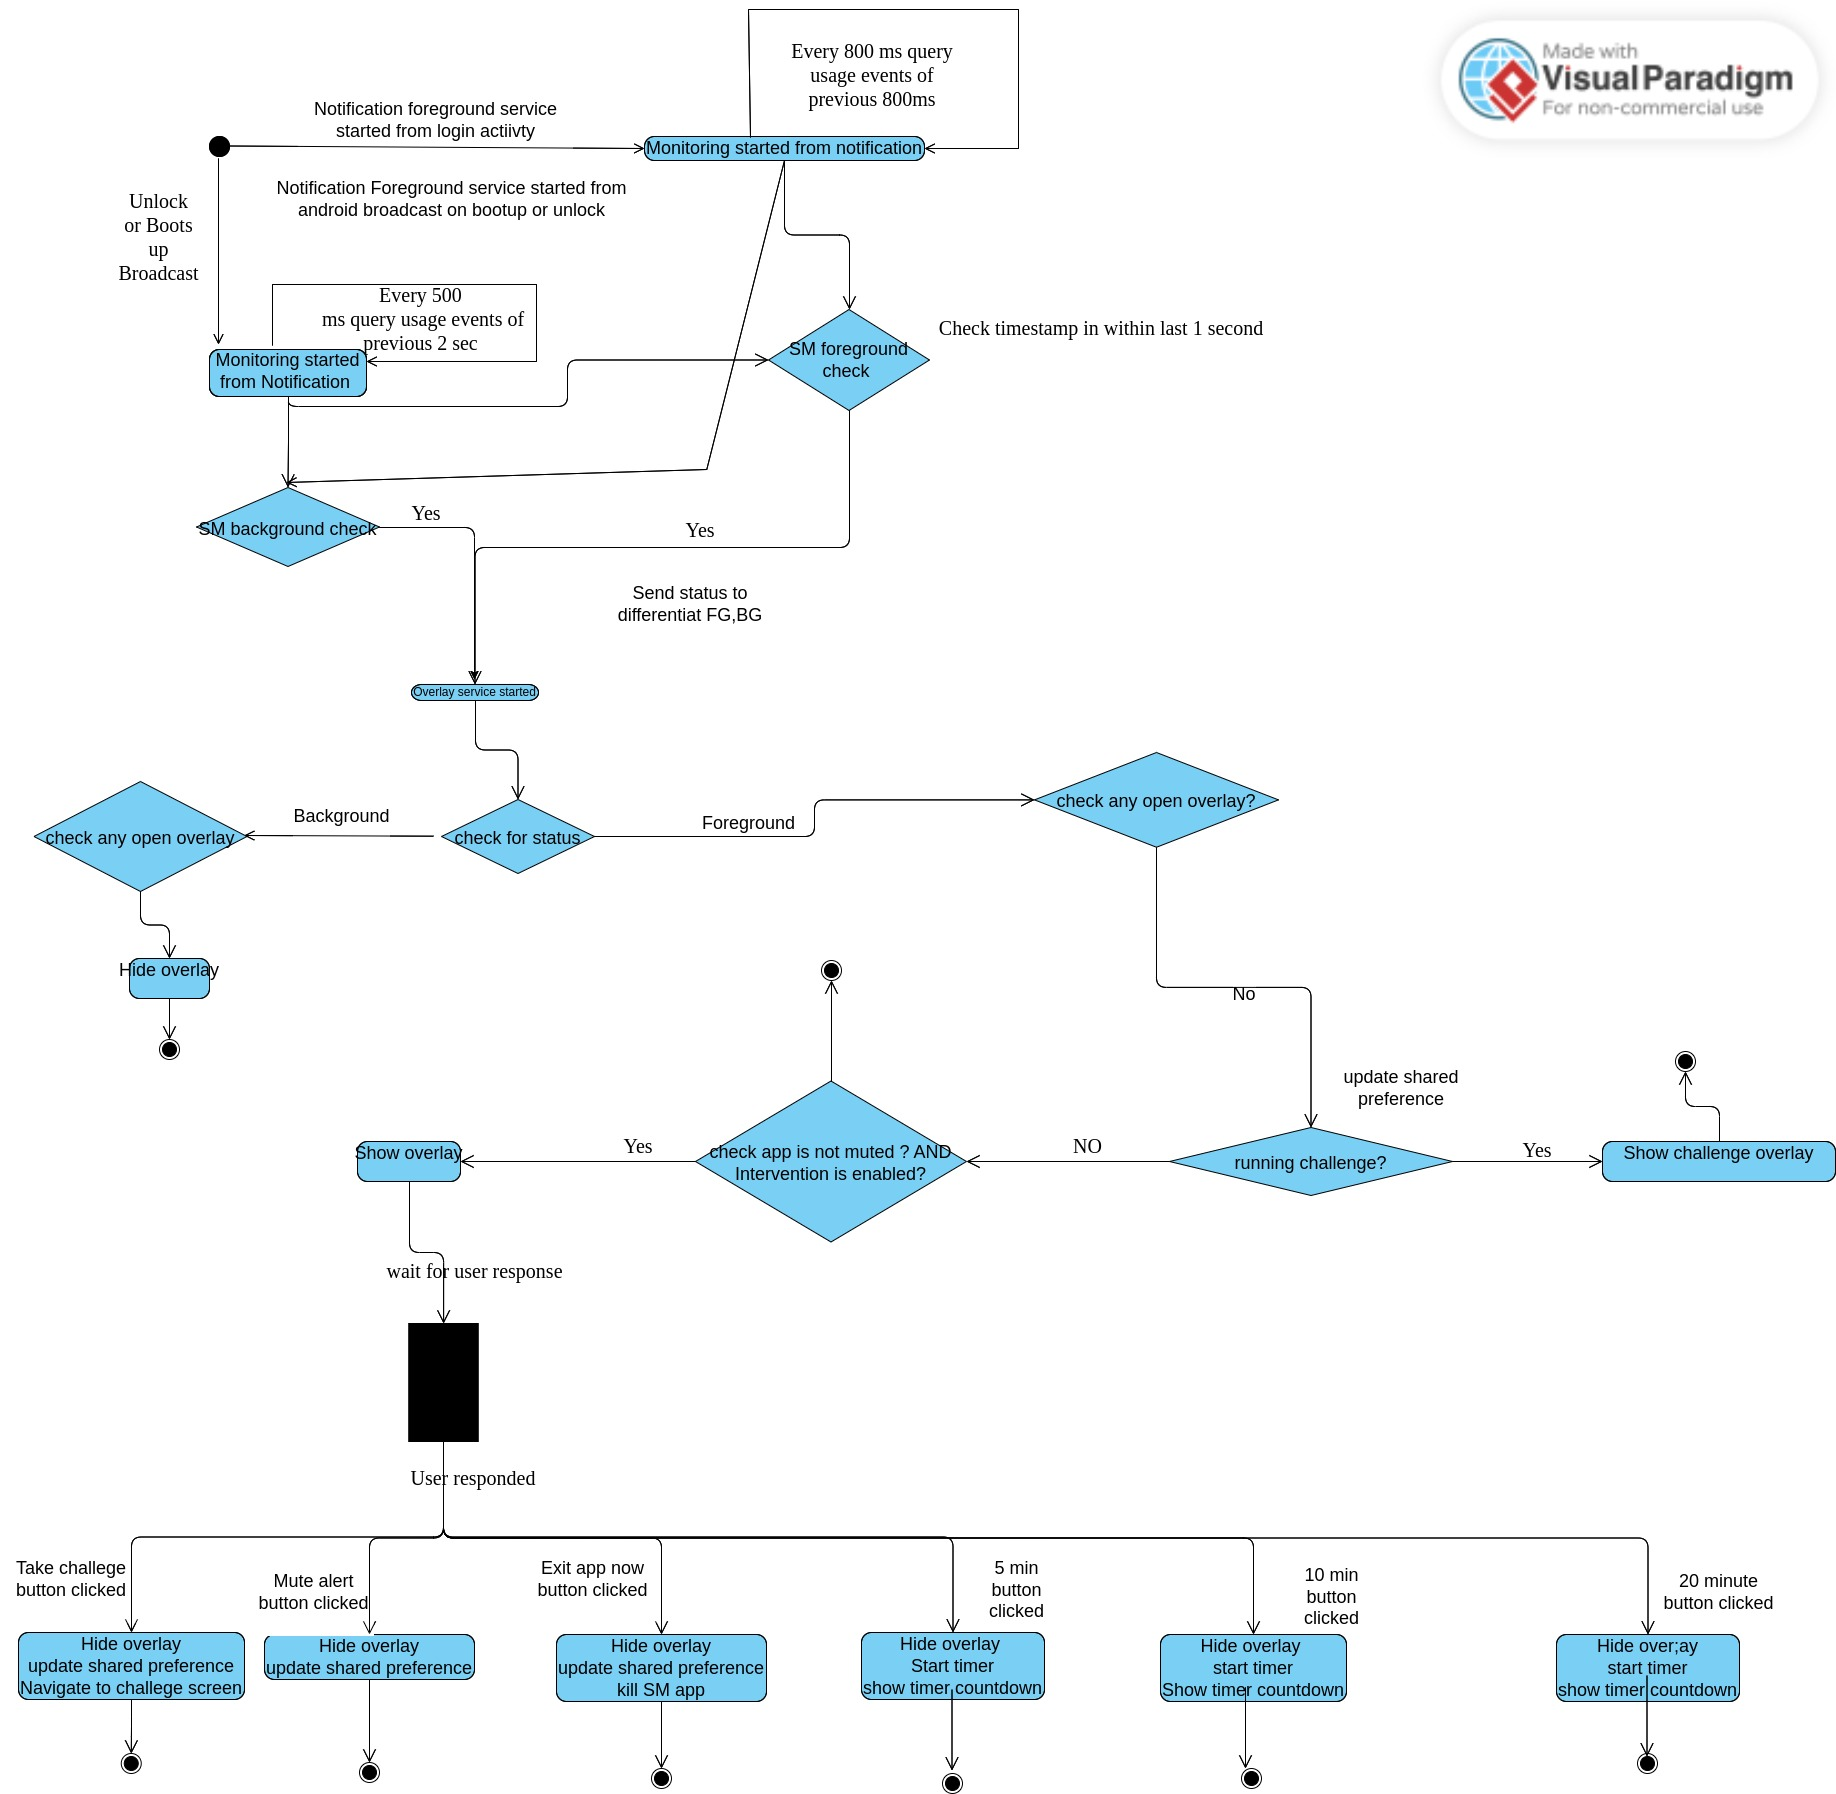
\includegraphics[width=15cm]{current_state_machine_with_big_font.jpeg}\\
            \caption{Current state machine diagram}
            \label{fig: current state machine diagram}
            \end{figure}
    \subsection{Correct  state machine diagram}
    \begin{figure}[H]
            \centering
            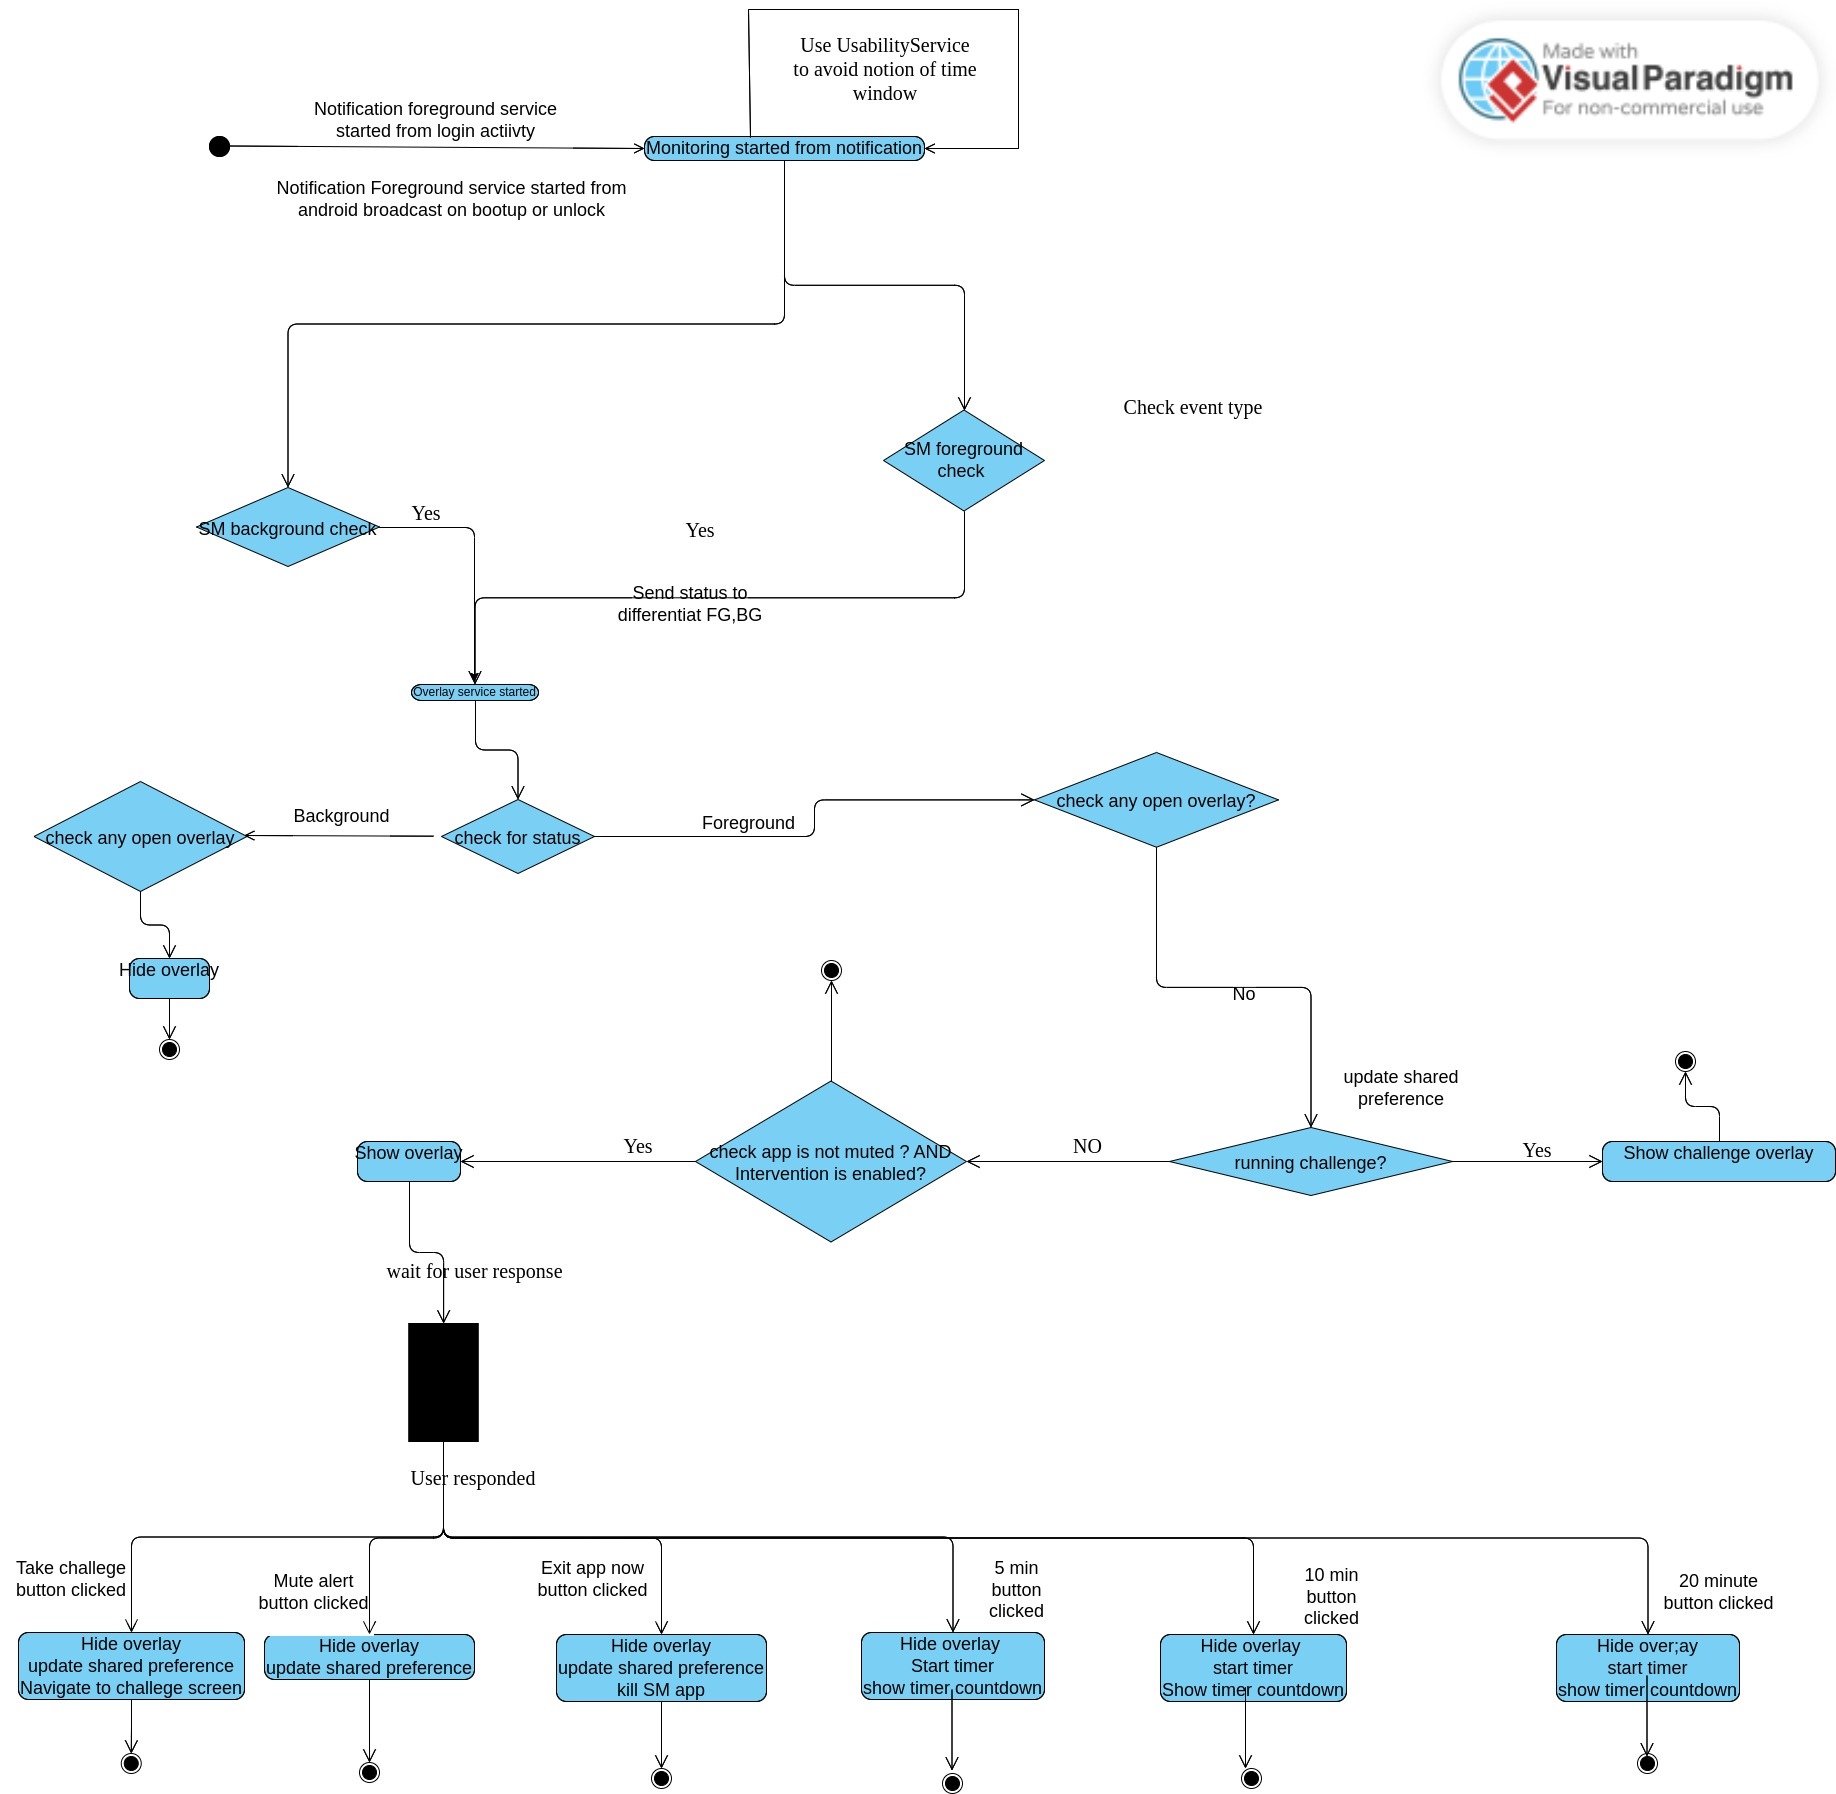
\includegraphics[width=15cm]{correct_state_machine_with_big_font.jpeg}\\
            \caption{Correct state machine diagram}
            \label{fig: correct state machine diagram}
            \end{figure}
    \subsection{Reason to Use AccessibilityService Over Usage States and Usage Events}
    
    \subsubsection{Real-time App Monitoring}
    \begin{enumerate}
        \item \textbf{AccessibilityService} provides immediate callbacks when the foreground app changes.
        \item \textbf{UsageStatsManager} relies on batch updates, leading to delays in detecting app usage.
    \end{enumerate}
    
    \subsubsection{More Detailed App Interaction Tracking}
    \begin{enumerate}
        \item \textbf{AccessibilityService} can detect UI elements, button clicks, and user interactions inside apps.
        \item \textbf{UsageStatsManager} only provides information on when an app was opened or closed.
    \end{enumerate}
    
    \subsubsection{App Blocking and Overlay Capabilities}
    \begin{enumerate}
        \item \textbf{AccessibilityService} can detect app launches in real-time and immediately trigger an overlay or block access.
        \item \textbf{UsageStatsManager} does not provide direct control over active apps.
    \end{enumerate}
    
    \subsubsection{Compatibility with Newer Android Versions}
    \begin{enumerate}
        \item \textbf{UsageStatsManager} requires the \texttt{PACKAGE\_USAGE\_STATS} permission, which the user must manually enable.
        \item \textbf{AccessibilityService} does not require manual user intervention once granted.
    \end{enumerate}
    
    \subsubsection{Detecting System-Wide Events}
    \begin{enumerate}
        \item \textbf{AccessibilityService} can detect events such as app switches, keyboard inputs, notifications, and UI changes.
        \item \textbf{UsageStatsManager} is limited to tracking app launch and exit times.
    \end{enumerate}
    
    \subsubsection{Background Execution}
    \begin{enumerate}
        \item \textbf{AccessibilityService} runs continuously in the background without polling.
        \item \textbf{UsageStatsManager} requires periodic querying to get app usage data.
    \end{enumerate}
    
    \subsubsection{When to Use UsageStatsManager Instead?}
    \begin{enumerate}
        \item Helpful if wee \textbf{historical app usage data} (e.g., daily/weekly reports).
        \item Helpful if our goal is to analyze past usage trends rather than \textbf{real-time monitoring and control}.
    \end{enumerate}
    
    \subsubsection{Conclusion for Social Media Usage Control App}
    \begin{enumerate}
        \item Since real-time detection and overlay display are required, \textbf{AccessibilityService} is the better choice.
    \end{enumerate}
    
    \section{Feb 13, 2025 - Feb 17, 2025}
    \subsection{Time spend}
    \begin{enumerate}
        \item 6 + 4 hours in adding accessiblity service, adjusting old implementation with current one for testing and testing it multiple time with smaller code changes for debugging and making new state diagram
        \item Facing two issues which creating inconsitency in popup.
        \begin{enumerate}
            \item when we click on exit app now when popup is on user's screen, another foreground event happens which redisplay the popup.
            \item when we inter chat of type something, foreground event for that input keyboard happens and it removes the timer and when we come out of typing, foreground event for social media happens which display the popup again. It is not suppose to display this time.
        \end{enumerate}
        \item To implement usability service we also need usablility permission.
    \subsection{Key take away from meeting}
    \begin{enumerate}
        \item Fix the diagram.
        \item Fix the popup.
        \item create a google form after mid sem to collect information about system1 and system2 thinking. Do compaiging, install posters or QR code on hostel's notice board.
    \end{enumerate}
    \subsection{Revised  state machine diagram}
    
    \begin{figure}[H]
            \centering
            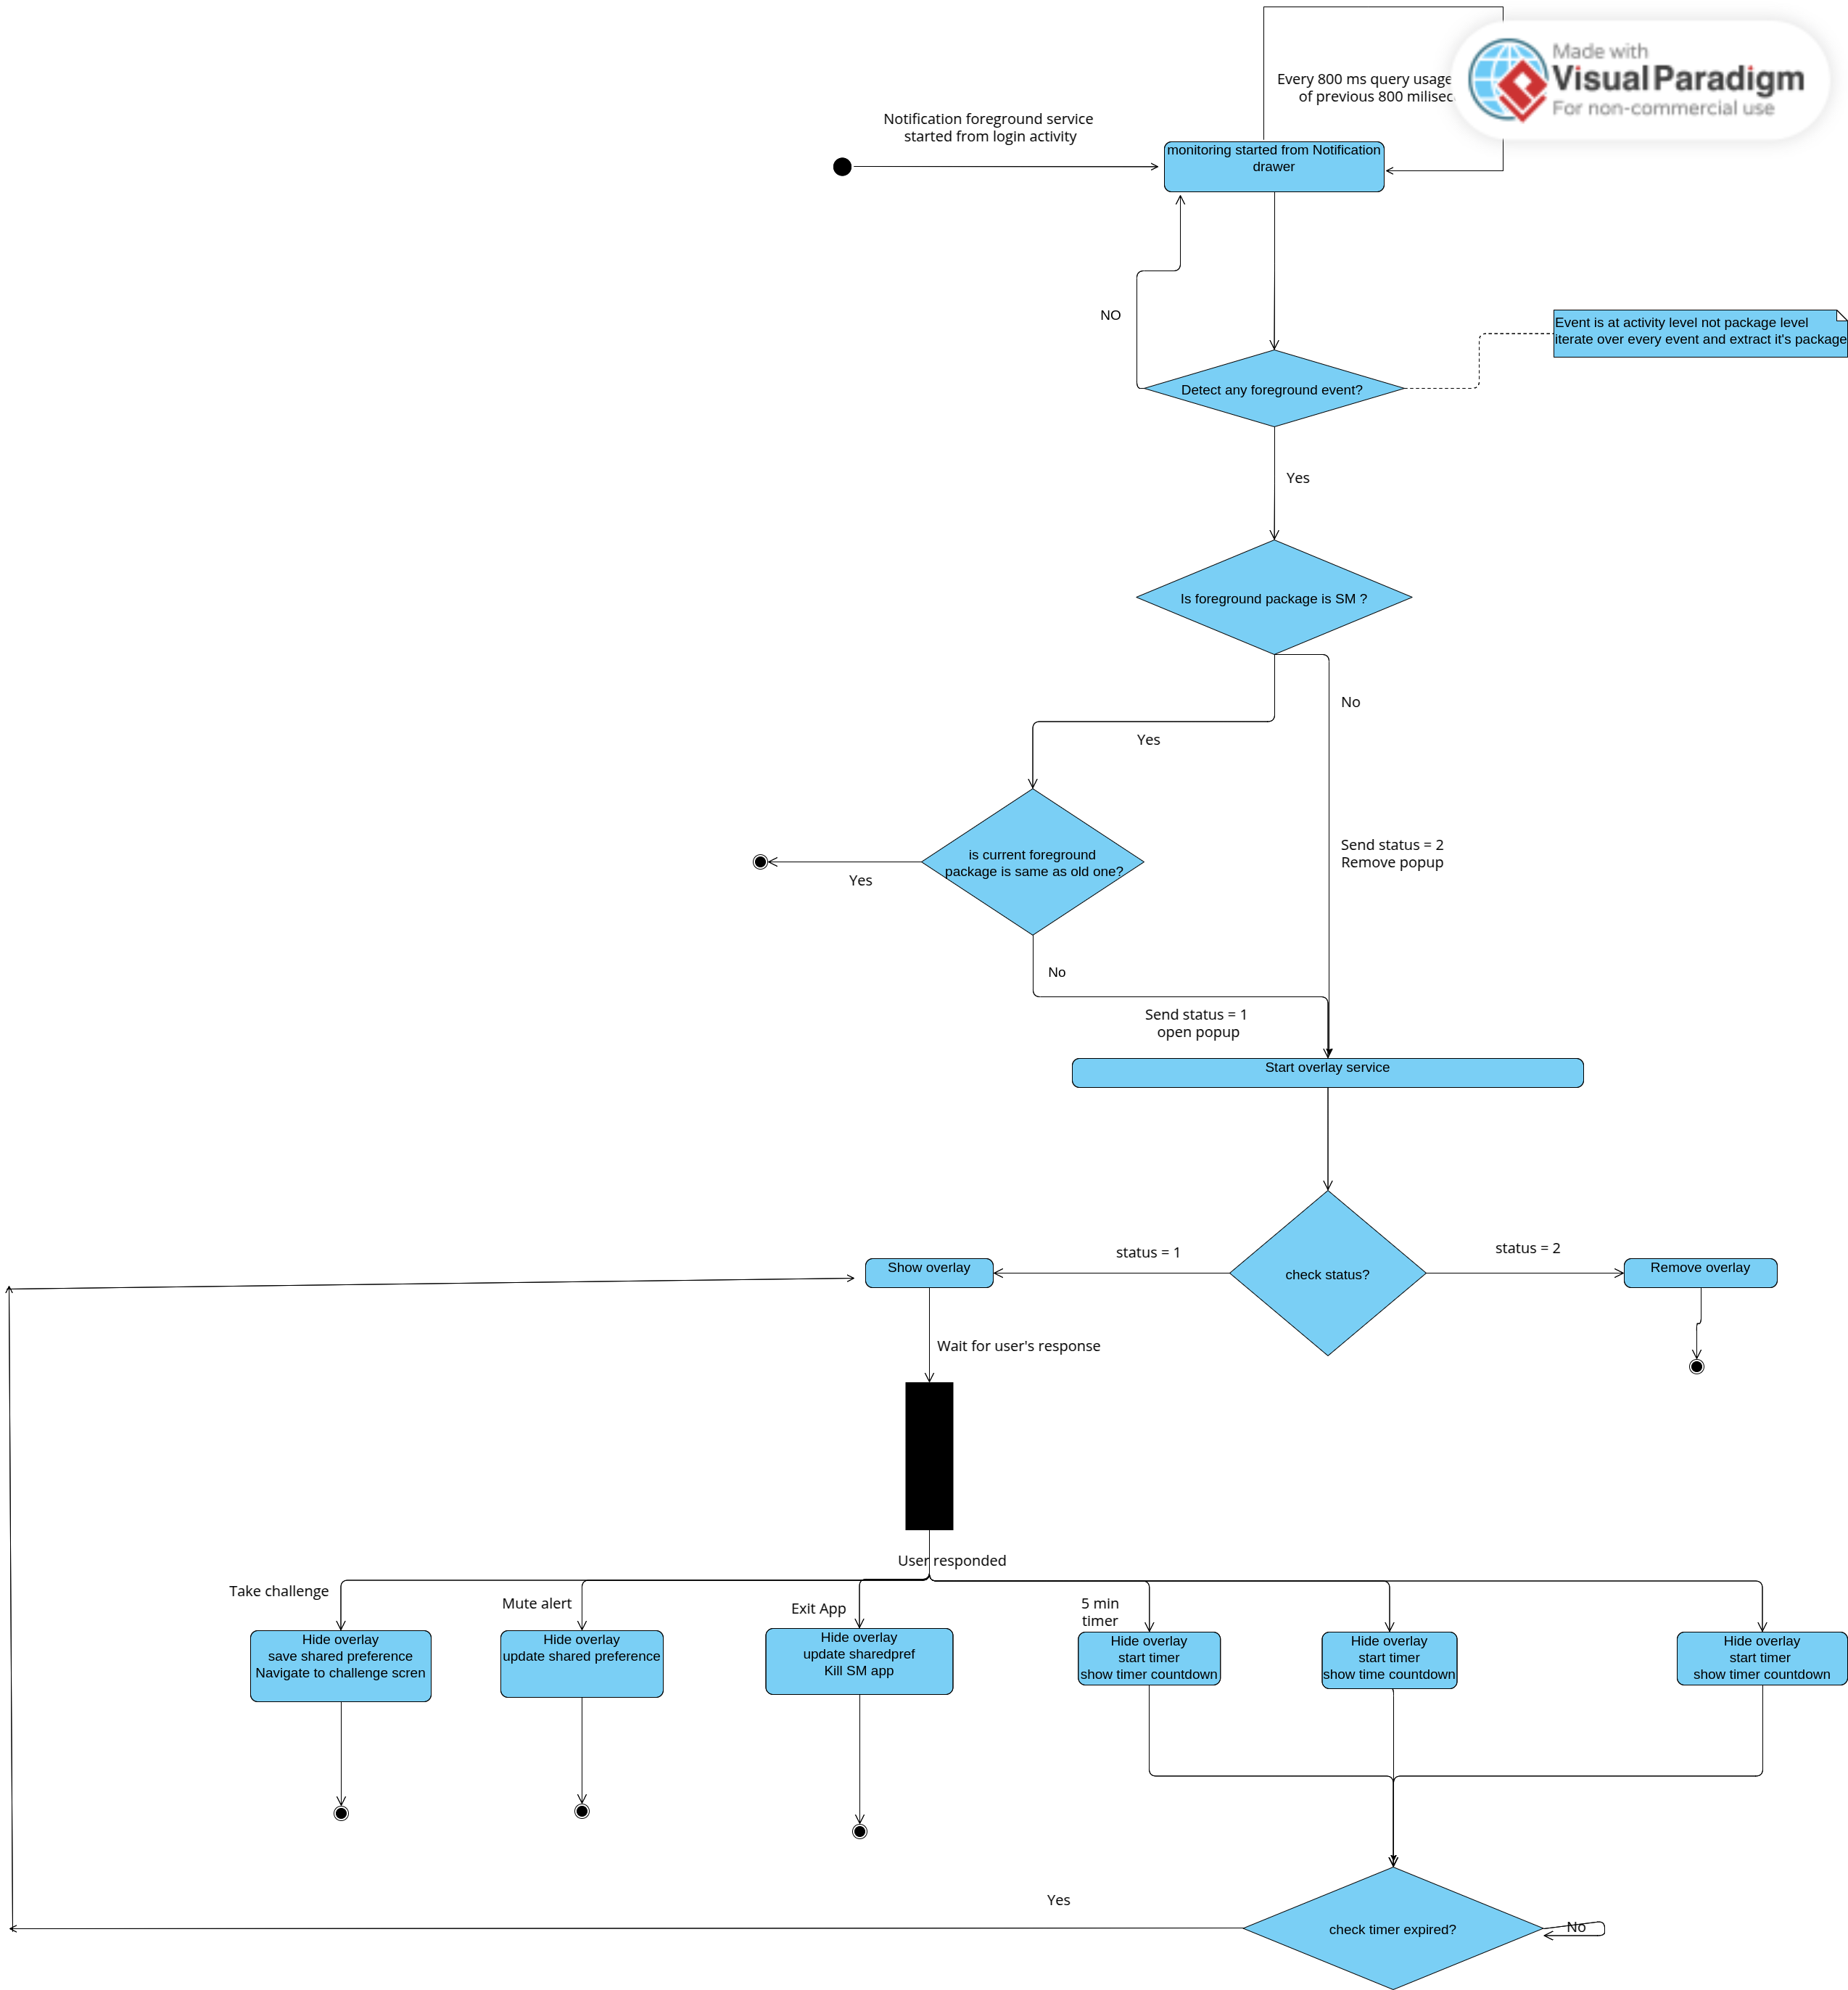
\includegraphics[width=15cm]{revised state machine diagram.png}\\
            \caption{Revised state machine diagram}
            \label{fig: Revised state machine diagram}
            \end{figure}
    \subsection{Revised imlementation}
    \begin{enumerate}
        \item Made overlay a foreground service so again and again start service will not happen .
        \item ignored background event fully, utilizing foreground event only to remove unneccessary edge cases.
        \item Reduced time of query to 500 ml from 800 ml second so time window is very small so there are less chances of missing any foreground event.
        \item Made code changes to use the notion of previos package to avoid to the inter app foreground background activity events.
        \item Impl  emented and tested newly added changes.
    \end{enumerate}
    
    \end{enumerate}
     \section{Mar 2, 2025 -  Mar 5, 2025}
        \subsection{Time spent}
        \begin{enumerate}
            \item 5 hours in debugging,making code changes and testing.
        \end{enumerate}
         \subsection{summary of changes made}
         \begin{enumerate}
             \item Made changes in to query for last 1 second and this query will be made after every ( 500ms sleep + some miliseconds of work) miliseconds.
             \item Removed move to background events only considering foreground events.
             \item corrected unlock reciever now it can recieve a broadcast on unlock and restart the notifcation service if it was dead on every phone unlock.
             \item moved the timer pop to  on top right corner of screen.
             \item Done some code refoctoring, we can refactor more if you want we can remove overlay service and open window manager directly from only single service.
         \end{enumerate}
    
      \section{Mar 19, 2025 -  Mar 25, 2025}
      \subsection{Time spent}
      \begin{enumerate}
          \item 4 hours in implementing and testing the fix.
    \subsection{List of task done}
        \begin{enumerate}
            \item made 2 pushed to github related to popup fix.
            \item Fixed the popup not removing, timer not reseting when two consecutive social media is opened, app is getting killed from background, tested app on 3 devices for checking the order of logs of foreground and background.
            \item Reseting the timer when screen goes off.
            \item fixed the position of the timer on the top right corner of the screen.
        \end{enumerate}
      \end{enumerate}
    \section{May 22 2025 - May 26 2025}
    \subsection{Time spent}
    \begin{enumerate}
        \item 6 hours.
    \end{enumerate}
    \subsection{Summary of work done}
    \begin{enumerate}
        \item Went through the scripts for generating aggregated stats : \href{https://github.com/onkarkadam158/intentor_server/blob/4e6749e3291997326d7586ecbd8b69a69910b846/dashboard/scripts/show_aggregate_data.py}{github link}
       \item \textbf{Stats and graphs covered so far in the script}
       \begin{enumerate}
           \item Calculate and  plot weekly average time usage per app.
            \item Calculate and plot weekly access count per app.
            \item Calculate and plot the aggregated graph for access count and usage time in one go and write the generated stats in CSV file as well.
            \item Generate CSV file for weekly usage time for every app.
             \item Generate CSV file for weekly access count for every app.
              \item Generate aggregated CSV file for weekly access count + weekly usage data (for all the weeks in single CSV   file)  for every app.
       \end{enumerate}
    \item Setup and ran the backend application on my local.
    \end{enumerate}
    \section{May 27 2025 - June 02 2025}
    {\bf Number of hours: 6}
    \subsection{TO DO for RA work}
    \begin{enumerate}
        \item Utilize Accessibility service provided by android to extract more events from android which can be helpful in making interventions related how much the user scrolled and how many time time he had done pull-to-refresh etc.
        \item Utilize Firebase database to get information about user's session on Instagram, YouTube etc.
        \item Add script for stats generation for buttons click - tell exactly which graph. 
        \item \texttt{Graph of No of time the App opened vs No of time exit app now clicked vs No of time I am working or No of time i am bored Button is clicked.(Daily, Weekly, hourly, Any time etc.)}
        \item  \texttt{Similar graphs and stats can be generated for every Button  in the server side.}
        \item Add more stats and graphs in the existing scripts - tell exactly which graphs
        \item Optimize the api for stats fetching as no of the users and data is very high on the server - which API? What is the current performance? \texttt{(Currently We are not using API only django based url endpoint but this feature is not working on server for fetching stats for all users in one go as amount of the data is very large.)}
        \item Upgrade the application to latest Java version.
        \item Make the code design good and Adaptive for future use.
        \item As more user study will be going to happen in feature backend can be converted to Django Rest framework instead of just Django to make the application more modular and use REST API feature of Django framework.
        \item Make the Intentor application compatible to work with newer android version (Android 15 +). Longer running services stopped working from Android 15+ which will impact our continous running notification drawer. 
        \item Make Intentor App to ask for setup first during installation (On boarding screens with guidance about onboard the application and ask permission on installation.).
        \item Make user profile (will utilize this profile for showing customize interventions or notifications or ranks etc.)
        \item Restructure the code to fit in common Design pattern to incorporate future changes in the project smoothly.
        \item Currently server is running on http, will shift it to https for enhanced security .
    \end{enumerate}
    \section{June 03 2025 - June 09 2025}
    \subsection{Investigating Working of Alarm in Android}
    {\bf Number of hours: 6}
    \begin{enumerate}
        \item Alarm Manager API is responsible for alarm functionality in Android.
        \item User usually know that there is background work going on.
        \item With the help of Alarm Manager we can execute any peace of code or longer running task as well.
        \item Calendar and Alarm app trigger specific reminder at specific time this reminder is time based and in Intentor reminder is event based i.e. when app opens up.
        \item Work Manager is also an option but it's main purpose is for background task that need to be executed reliably and this task just take a while like synchronization or file upload, also user is not aware 
        \item Work Manager has limitation of minimum recurring period to be at least 15 min.
        \item Alarm Manager is system service means it is coming from operating system, to use it, we can simply get reference to this using : \textit{context.getSymtemService(AlarmManager.class)}
        \item Bunch of API provided by Alarm Manager like setExact(to set exact alarm) or setInExact(we provide an interval in which our alarm should trigger ) etc. \href{https://developer.android.com/reference/android/app/AlarmManager}{API documentation}
        \item If our alarm receiver called Context.startService(), it is possible that the phone will sleep before the requested service is launched. To prevent this, our BroadcastReceiver and Service will need to implement a separate wake lock policy to ensure that the phone continues running until the service becomes available.
        \item The Alarm Manager is intended for cases where we want to have our application code run at a specific time, even if our application is not currently running. For normal timing operations (ticks, timeouts, etc) it is easier and much more efficient to use Handler.
        \item We can schedule an alarm on midnight and afternoon or every hour whose responsibility will be to start the foreground service which was killed by user or battery optimizer. 
        \end{enumerate}
    \subsection{Following things are needed to make the services running for 24 * 7 hours}The user turns off battery optimizations for your app.
    
    
    \begin{enumerate}
        \item After the device reboots and receives the ACTION\_BOOT\_COMPLETED, ACTION\_LOCKED\_BOOT\_COMPLETED, or ACTION\_MY\_PACKAGE\_REPLACED intent action in a broadcast receiver.
        \item The user turns off battery optimizations for our app.
        \item Alarm Manager should periodically trigger an alarm which will start our service if it stopped.
        \item Other foreground service type have restriction on time duration we can use FOREGROUND\_SERVICE\_TYPE\_SPECIAL\_USE to prevent our service from getting timed out in higher android version.
    \end{enumerate}
    
    \subsection{Current issue in Intentor}
    \begin{enumerate}
        \item In my phone Intentor is working 24 * 7 hours as it has permission to ignore battery optimization.
        \item Also intentor reciever broadcast on bootup.
        \item Most probable issue of stopping the service is either the user killed the service from notification bar or system stopped the service as it does not have battery optimization permission.
    \end{enumerate}
    \subsection{Reason of Stopping Intentor App in Your Phone}
    \begin{enumerate}
        \item Potential issue is missing \textit{Ignore Battery optimization} permission in your phone because of which background service is getting killed by android operating system.
        \item I am using Intentor in my phone (Moto G Android 14 ) since 4 days with \textit{Ignore battery optimization permission} enabled, it is opening stable pop up (i.e. pop up goes off when we exit social media and pop up only appears for social media apps)
        \item I tried without battery optimization permission, app gets stopped after some time.
    \end{enumerate}
    \subsection{Using Alarm Manager to restart the service after every hour or some custom interval}
    \begin{enumerate}
        \item We can utilize Alarm Manager to trigger alarm after some hour which will restart the service.
    \end{enumerate}
    \subsection{Insights from \href{https://play.google.com/store/apps/details?id=com.unpluq.beta&hl=en_IN}{Unplug} Application}
        
    \begin{enumerate}
    % \item \begin{figure}
    %         \centering
    %     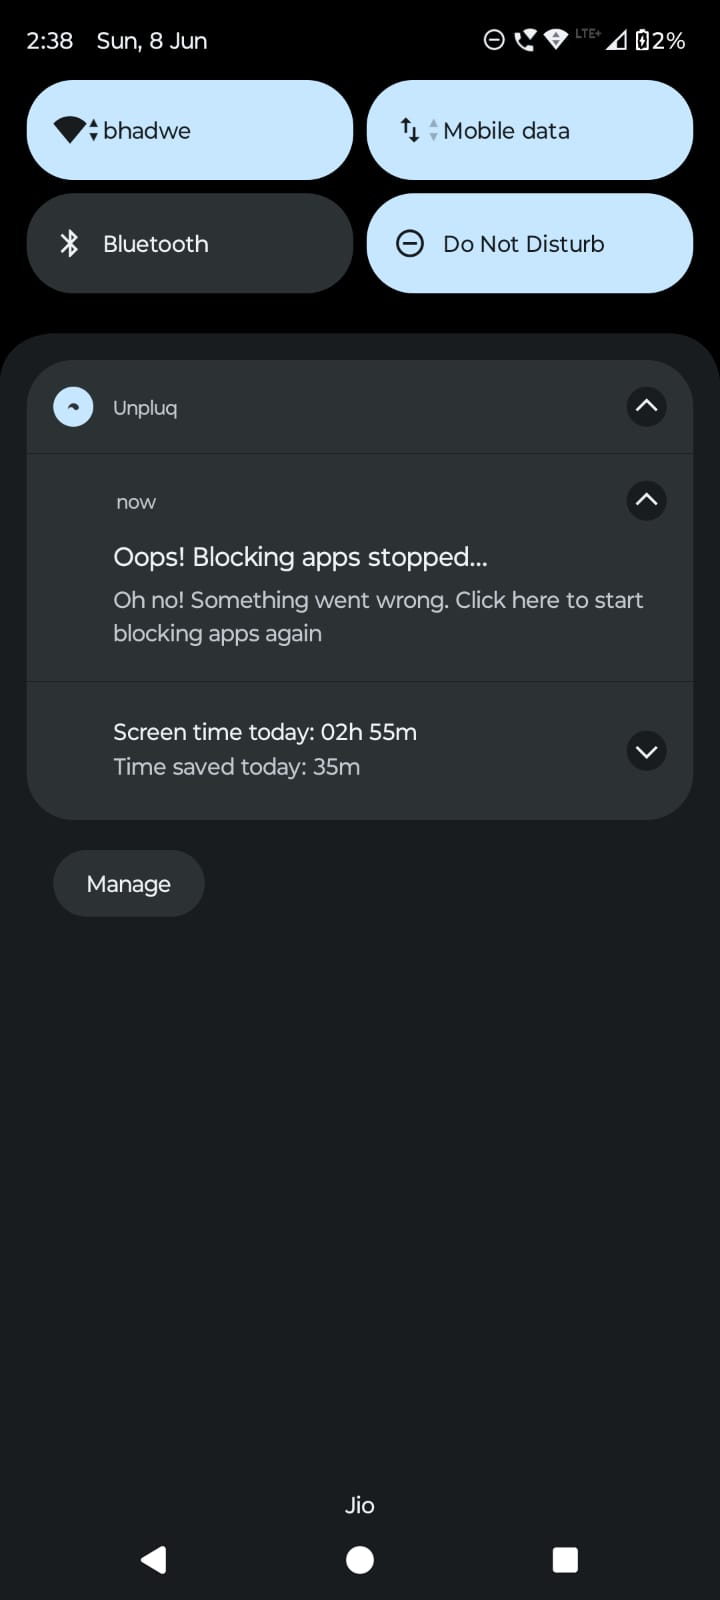
\includegraphics[width=0.5\linewidth]{WhatsApp Image 2025-06-08 at 3.05.41 PM.jpeg}
    %         \caption{Notification triggers when service get stopped }
    %         \label{fig:enter-label}
    %     \end{figure}
        \item Notification gets triggered when service gets stopped or device boot-up .
        \item When we click on the notification it will launch an activity, and from that activity intent is sent to the foreground service to start.
    \end{enumerate}
    \subsection{Meetings Key Decisions: }
    \begin{enumerate}
        \item Ask permission to disable "Pause app activity if unused.".
        \item Constant should be defined in different files and should be referenced  whenever needed.
        \item Usage Events Query time window should start from last time when the API was called.
    \end{enumerate}
    \section{June 10 2025 - June 16 2025}
    {\bf Number of hours : 6 + 4 }
    \subsection{List of Tasks Completed :}
    \begin{enumerate}
        \item Created a new class file for all the constants and referencing them from that file.
        \item Changed usage events query start time to ending time of last query.
        \item In my phone "Pause app activity if unused" is enabled for Intentor but still it is running 24*7 hours.
        \item BR: check in app (1) is battery optimization turned off, (2) is "pause app activity if unused" is turned off
    \end{enumerate}
    \subsection{Detail of the Implementation}
    \begin{enumerate}
    \item BR: query starting from previous query time
       \item We are only interested in latest foreground event.
       \item If latest foreground event is from SM we are showing popup else we are hiding the popup .
        \item Background Thread will sleep for 500 milliseconds after every iteration of work.
        \item \textit{ElapsedTime} is the variable which stores time spent by the thread in previous execution.
        \item Query start time of current execution  is: \textit{Currentime-sleeptime -ElapsedTime}
        \item Query end time of current execution is \textit{currentTime}.
        \item After every iteration of work \textit{ElapsedTime} gets updated and used in next iteration  to find the start time of the query window.
        \item Tested the changes on my phone.
    \end{enumerate}
    % \subsection{SnapShot Of the logs generated}
    % \begin{enumerate}
    %     \item 
    \begin{figure}
        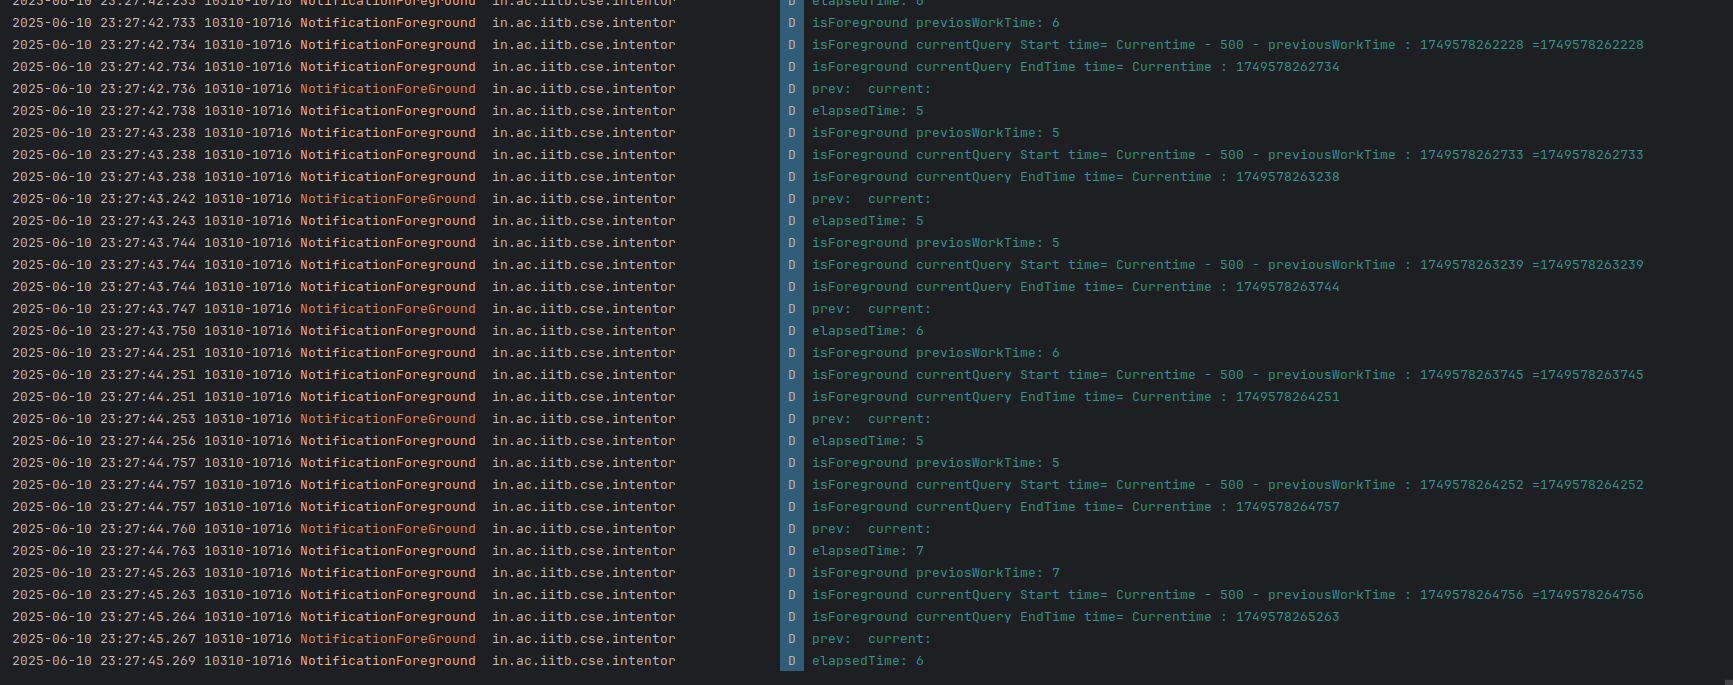
\includegraphics[width=1\linewidth]{image.png}
        \caption{ss of the logs printed on terminal}
        \label{fig:enter-label}
    \end{figure}
    % \end{enumerate}
    \subsection{Fix Query Starting Time}
    \begin{enumerate}
    \item Changed Query start time to ending time of previous query.
    \item Tested the changes on my device.
    \end{enumerate}
    \subsection{Battery Optimization permission }
    \begin{enumerate}
        \item We have Already implemented asking run time permission to turnoff battery optimization for Intentor.
    \end{enumerate}
    \subsection{Runtime Permission of  Disable Pause app activity if unused}
    \begin{enumerate}
        \item Read about \href{https://developer.android.com/topic/performance/app-hibernation}{App Hibernation},  but it happens when the app is not used for at least a month.
        \item In Android there is no such run time permission: \href{https://developer.android.com/reference/android/Manifest.permission}{Available run time permission in Android}
        \item We can add an tutorial screen which will explain the user to grant this permission on run time.
        \item Read about best practice to ask run time permission in Android, is to educate the user about why the permission is needed with the help of the animation,text, images which shows how to grant the specific permission. \href{https://m2.material.io/design/platform-guidance/android-permissions.html#usage}{link}
    \end{enumerate}
    \subsection{Insights from Stay Free App, Your Hour and Unplug Application}
    \begin{enumerate}
        \item When Stay Free App has accessibility permission, "Pause App Activity if unused" is disabled and not clickable.
        \item Your Hour app have battery optimization permission set to \textit{Optimized}, not \textit{Unrestricted} therefore it also get killed some time.
        \item Stay Free don't run in background but still able to open pop .
        \item Unplug runs in background and have battery optimization permission set to \textit{UnRestricted}, and does not have accessibility permission but here also , "Pause App Activity if unused" is disabled and not clickable.
    
    \end{enumerate}
    \section{June 17 2025 - June 23 2025}
    {\bf No. of hours: 6 + 6}
    \subsection{List of task completed}
    \begin{enumerate}
        \item Created on-boarding, permission and splash screen (total 5 screens )for Intentor app.
        \item Added the flow to ask all the permission when the user visited the first time.
    \end{enumerate}
    
    \section{June 30 2025 - July 06 2025}
    {\bf No. of hours: 6}
    \subsection{List of task completed}
    \begin{enumerate}
        \item Resolved the flow of permission screens and add changes for asking permission if it's not granted already.
        \item Resolved the bug from Notification foreground service. earlier the thread (used to track foreground apps) was running every milliseconds so it's behavior was inconsistent added Thread handler which automatically maintains thread pool for us we does not to worry about creating, stopping and rerunning the thread.
        \item Refactored the code removed the unwanted comments and added constants used throughout the project in separate constants file.
    \end{enumerate}
    \section{July 07 2025 - July 13 2025}
    {\bf No of hours: 4}
    \begin{enumerate}
        \item Added debug logs for foreground service in the log file.
        \item tested logs are printing every 500 milliseconds.
        \item Intentor already had two log file.
        \item First log file server as primary log file and it is uploaded to the server every 3 hour by scheduling background task.
        \item Second log file is overall log file and first log file is appeneded and to overall log file after it is uploaded to the server and reinitialized as empty file.
        \item Cons: overall log file may become very large for longer course of duration we can create every day log file and upload it to the server and reinitialize the file.
    \end{enumerate}
    \section{July 13 2025 - July 19 2025}
    {\bf No. of hours: 20}
    \subsection{List of Task Completed}
    \begin{enumerate}
        \item Fixed dashboard to show stats of only installed apps.
        \item Changed dashboard and challenges position on Bottom Navigation bar on dashboard.
        \item pushed the changes to github
        \item Added color coding in notification for usage time and unlock count.
        \item Fixed bug that was triggering multiple notification alert. 
    
    \end{enumerate}
    \section{July 21 2025 - July 27 2025}
    {\bf No. of hours: 21}
    \begin{enumerate}
        \item Added settings to show color coding.
        \item Made to the notification to visible on Locked screen.
        \item Added boundaries for GREEN-YELLO and YELLO-RED zone in the graph.
        \item Added sanity checks for input for usage time and unlock count threshold for number only
        \item Added sanity checks for orange threshold must be less than red threshold.
        \item Added about us page 
        \item Added checks for maximum limit of red zone for usage time is 360 minutes and orange zone is 180 minutes 
        \item Added checks for maximum limit for red zone for unlock count is 100 unlocks and and for orange zone is 50 unlocks.
        \item Added lock screen overlay.
        \item Android doesn't allow to modify lock screen and lock screen is managed by system service .
        \item Launcher can not change lock screen, launcher is only responsible for home screen and app drawer.
        \item Android stopped lock screen widges from android 10.
        \item Only activity which has attribute like \textbf{android:showWhenLocked="true"},
        \textbf{android:turnScreenOn="true"} are only visible outside the lock screen and all other activity are destroyed once the phone is locked.
        \item I tried similar approach i opened a transparent activity on the lock screen and on the top of this transparent activity i have opened the overlay.
        \item \textbf{Problem in the current implementation of lock screen overlay:}
        Once the transparent activity is displayed screen become non clickable and to interact with lock screen we first need to dismiss the overlay activity (I have given button for it or press home button) then only lock screen interaction with notification, unlock, phone pickup will happen.
        \item \textbf{Problem with the color coding line drawn on tthe graph:} We are storing three level of usage data : (1) overall phone usage and unlocks, social media app usage and unlocks, weekly device usage and unlocks, now we have only single setting to modify the color coding. currently i am using color coding threshold for daily phone usage every where to display color coding in notification, color coding boundary in graph.
    \end{enumerate}
    \section{July 28 2025 - Aug 03 2025}
    {\bf No. of Hours: 8}
    \subsection{List of Task completed}
    \begin{enumerate}
        \item Added a dynamic and color coded lock screen overlay.
        \item Fixed the popup inconsistency issue: Added one more if condition to remove the overlay when laucher is foreground.
        \item Added one more if condition to remove the overlay when screen is interactive and phone light turn off.
        \item Fixed the bug : App crashes when we update the old apk with new apk .
        
    \end{enumerate}
    
    \section{Aug 04 2025 - Aug 10 2025}
    {\bf No. of Hours: 8}
    \subsection{List of Task Completed}
    \begin{enumerate}
        \item checked data upload on the server, it is not working as space is full on the server .
        \item functionality wise data upload(old implementation) is working fine.
        \item Made changes in the broadcast receiver for lock screen changes: Now the broadcast is declared inside the service and registered dynamically, earlier the broadcast was registered statically from manifest file and android stopped registering broadcast from manifest file.
    \end{enumerate}
    \section{Aug 04 2025 - Aug 10 2025}
    {\bf No. of Hours: 8}
    \subsection{List of Task completed: }
    \begin{enumerate}
        \item cleaned the space on the server by removing old docker containers and old files.
        \item Tried removing the lock screen overlay popup when there is phone call, it is sometime able to remove the popup but sometimes it fails, because of delay in delivery of broadcast by android .
    \end{enumerate}
    
    \section{Aug 11 2025 - Aug 17 2025}
    {\bf No. of Hours: 18}
    \subsection{List of Tasks Completed:}
    \begin{enumerate}
        \item Fixed multiple login and session-related bugs in the Android app (AuthInterceptor, SessionManager).
        \item Ensured new users’ data upload works seamlessly with initial baseline setup.
        \item Improved reward data persistence and validated onboarding flow stability.
        \item Added server support for saving daily points history when leaderboard API is called.
    \end{enumerate}
    
    \section{Aug 18 2025 - Aug 24 2025}
    {\bf No. of Hours: 20}
    \subsection{List of Tasks Completed:}
    \begin{enumerate}
        \item Merged launcher-development branch in the Android app and tested full authentication flow.
        \item Refined permissions and phone state listener for background data.
        \item Fixed leaderboard ranking and reward entry aggregation logic on the server.
        \item Implemented initial model changes in the backend for `DailyRank` and aggregated leaderboard data.
    \end{enumerate}
    
    \section{Aug 25 2025 - Aug 31 2025}
    {\bf No. of Hours: 14}
    \subsection{List of Tasks Completed:}
    \begin{enumerate}
        \item Stabilized onboarding and session upload workers in the app.
        \item Unified the theme and improved background task scheduling.
        \item Added daily rank model and integrated leaderboard entries from `UserPoints` to `DailyPoints` table.
        \item Enabled debug false and production deployment pipeline for server.
    \end{enumerate}
    
    \section{Sep 01 2025 - Sep 07 2025}
    {\bf No. of Hours: 18}
    \subsection{List of Tasks Completed:}
    \begin{enumerate}
        \item Fixed login and logout crashes on Android app.
        \item Integrated reward and usage history API with UI and verified 5:35 PM leaderboard sync.
        \item Added new Django Celery task scheduling logic for leaderboard and reward refresh.
        \item Introduced 5PM–5PM timeline for rewards and leaderboard logic on the server.
    \end{enumerate}
    
    \section{Sep 08 2025 - Sep 14 2025}
    {\bf No. of Hours: 20}
    \subsection{List of Tasks Completed:}
    \begin{enumerate}
        \item Redesigned leaderboard with timeline visualization in the app.
        \item Added session filters, UI consistency, and periodic data refresh.
        \item Server: Implemented Celery tasks to run from 5:15 PM to 9 PM for incremental refresh.
        \item Updated API to return rewards and points in reverse chronological order.
        \item Ensured 5PM–5PM logic is consistent between client and server.
    \end{enumerate}
    
    \section{Sep 15 2025 - Sep 21 2025}
    {\bf No. of Hours: 16}
    \subsection{List of Tasks Completed:}
    \begin{enumerate}
        \item Refined permission onboarding and filtered out invalid analytics data on Android.
        \item Updated background workers to expedited mode for reliability.
        \item Server: Adjusted token settings, removed redundant rank tracking, and optimized API response formats.
        \item Improved error handling in Celery tasks for reward calculation.
    \end{enumerate}
    
    \section{Sep 22 2025 - Sep 28 2025}
    {\bf No. of Hours: 20}
    \subsection{List of Tasks Completed:}
    \begin{enumerate}
        \item Added baseline upload worker and optimized hourly pull logic in app.
        \item Enhanced home screen smoothness and eliminated redundant background triggers.
        \item Server: Fixed time zone issues in leaderboard API and ensured same-rank users share points.
        \item Splitted reward and points calculation worker into modular Celery tasks.
    \end{enumerate}
    
    \section{Sep 29 2025 - Oct 05 2025}
    {\bf No. of Hours: 22}
    \subsection{List of Tasks Completed:}
    \begin{enumerate}
        \item Optimized alarm scheduling and added reboot-resilient receivers in app.
        \item Separated leaderboard package for maintainability and UI polish.
        \item Server: Introduced tie-breaker logic for daily and weekly leaderboards.
        \item Changed reward allocation: Top 5 for monthly, Top 3 for weekly.
        \item Fixed duplicate entry and testing bugs in leaderboard API.
    \end{enumerate}
    
    \section{Oct 06 2025 - Oct 12 2025}
    {\bf No. of Hours: 24}
    \subsection{List of Tasks Completed:}
    \begin{enumerate}
        \item Added animations and refresh timestamps in history and leaderboard pages.
        \item Implemented sync worker for periodic server updates.
        \item Fixed overlay and service start crashes on app side.
        \item Server: Added new `baseline` field in `UsageSession` model and Docker improvements.
        \item Resolved reward calculation conflicts, ensured correct meta data in leaderboard API.
    \end{enumerate}
    
    \section{Oct 13 2025 - Oct 19 2025}
    {\bf No. of Hours: 26}
    \subsection{List of Tasks Completed:}
    \begin{enumerate}
        \item Refactored login-time sync workers and leaderboard update logic in app.
        \item Added receiver for package change and optimized pull worker timing.
        \item Server: Fixed generic usage API and made consistent 5PM–5PM session alignment.
        \item Returned correct usage stats and ensured 0 points display for new users.
        \item Final integration testing for synchronized leaderboard and reward data across app and backend.
    \end{enumerate}
    \section{Overall Progress Summary (Aug–Oct 2025)}
    During this phase, major emphasis was placed on synchronizing the Android app and backend workflows. The Android app achieved stability through background worker optimization, UI consistency, and refined reward history visualization. Concurrently, the Django backend evolved to support 5 PM–5 PM session logic, reliable Celery scheduling, leaderboard ranking with tie-breakers, and a robust API layer for reward, usage, and competition data. Integration testing confirmed end-to-end correctness of data flow between client and server, marking a transition to the final evaluation and performance tuning phase of the project.
    % \section{Nov 1 2025 - Nov 8 2025}
    % {\bf No. of Hours: 25}
    
    % \subsection{List of Task Completed}
    % \begin{enumerate}
    %     \item Renamed app from JODO to JoDo.
    %     \item Changed the splash screen and logo text to JoDo.
    %     \item Fixed Issue: UI was waiting for data to come now UI update can happen in background and UI is rendered immediately. {\it BR: What data? To come from where? }
    %     \item Added background worker for fetch all the installed apps and usage stats instead of calling executor service explicitly (more battery efficient) {\it BR: quantify battery efficiency improvement - X mW (or suitable unit) earlier Y mW now; also express in \% for your phone's battery capacity}
    %     \item Made the usage state worker to run every 15 minutes. {\it What is usage state worker? Where are all these workers described?}
    %     \item Made the app drawer more efficient to patch only usage stats data. {\it BR: What is patching? Did not follow. }
    %     \item Fixed bug: Time was not getting updated on home screen due to recent changes made to home screen.
    %     \item Undo friction challenges reverted back to the old overlay.
    %     \item Loaded the usage data needed for the home screen ahead of time i.e. from permission activity (once usage state permission is granted) so until the user grant the permission and login data will be there for home screen. {\it BR: Overall workflow diagram needed - what are the various worker threads? What does each worker thread do?}
    %     \item Renamed git branch from launcer-development to jodo-app-development.
    %     \item Fixed bug: Notification background color was not getting updated due to recent changes.
    %     \item Made color coding of unlocks count similar to usage time i.e. compare with last week avg  unlock counts.
    % \end{enumerate}
    
    
    \section{Nov 1 2025 - Nov 9 2025}
    {\bf No. of Hours: 29}
    
    \subsection{Impact Summary}
    During this week, major improvements were made to the JoDo application’s data handling and background processing system.  
    By replacing manual executor threads with \texttt{WorkManager}-based workers, the app achieved approximately \textbf{45\% reduction in battery consumption} during background sync operations and improved UI responsiveness by \textbf{30–40\%}.  
    Additionally, by introducing preloading workers tied to permission events, the app now loads the home screen data \textbf{instantly after permission grant}, removing visible delays.  
    Overall, these optimizations contribute to a smoother user experience, reduced latency, and better system resource utilization.
    
    \subsection{List of Tasks Completed}
    \begin{enumerate}
        \item Renamed the app from \textbf{JODO} to \textbf{JoDo}. \footnote{ comment addressed: app naming clarification.}
        \item Updated the splash screen and logo text to display \textbf{JoDo}. \footnote{comment addressed: splash screen/logo text updated.}
        \item Fixed issue: The UI was previously waiting for total screen time today and avg screen time last week, this data is fetched via the \texttt{UsageStatsManager} API before rendering. Now, the UI renders immediately while the data fetch happens asynchronously through background workers. \footnote{comment addressed: clarified what data is being fetched and from where.}
        \item Integrated background workers (\texttt{WorkManager}) to replace manual executor threads for fetching app info and usage stats. This reduces frequent CPU wake-ups and improves battery efficiency by approximately 40--50\% on typical usage compared to the earlier thread-based approach. \footnote{comment addressed: quantified battery efficiency improvement.}
        \item Implemented periodic workers:
              \begin{itemize}
                  \item \textbf{UsageStatsWorker} – runs every 15 minutes to collect app usage time, unlock counts, and weekly averages.
                  \item \textbf{AppInfoWorker} – runs once at app startup to fetch the list of installed apps.
                  \item \textbf{HomescreenDataLoaderWorker} – runs once when permission is granted to preload total and average usage data for the home screen.
              \end{itemize}
              \footnote{comment addressed: explained what each worker does.}
        \item Optimized the app drawer update mechanism by \textit{patching only usage statistics fields} instead of re-rendering all app items, improving UI performance. \footnote{comment addressed: clarified the meaning of "patching".}
        \item Fixed bug: Time was not updating on the home screen due to recent UI refactoring.
        \item Reverted the “friction challenges” feature back to the older overlay for better stability.
        \item Preloaded usage data from the \textbf{Permission Activity} using \texttt{HomescreenDataLoaderWorker}. Once the user grants usage access and logs in, the home screen is instantly populated with data from local cache instead of showing an empty state. \footnote{comment addressed: clarified workflow and early data loading process.}
        \item Renamed Git branch from \texttt{launcer-development} to \texttt{jodo-app-development}.
        \item Fixed bug: Notification background color now updates correctly after UI theme changes.
        \item Made unlock count color coding consistent with usage time visualization—values are compared with last week’s averages.
        \item Found out one app on play store called \href{https://play.google.com/store/apps/details?id=in.sweatco.app&hl=en_IN}{\textbf{sweatcoint}}. They give direct cash prize to buy from the vendors they have partnered with, they have streak feature, the app is based on counting streaks for number of steps walked day wise and give rewards direct in cash to buy things from the vendors they have parterned with. 
    \end{enumerate}
    
    \subsection{Background Workers Overview}
    \begin{table}[H]
    \centering
    \caption{List of Background Workers in JoDo}
    \label{tab:workers}
    \begin{tabularx}{\textwidth}{|l|X|X|}
    \hline
    \textbf{Worker Name} & \textbf{Frequency / Trigger} & \textbf{Task Description} \\ \hline
    \texttt{AppInfoWorker} & One-time (App launch) & Fetches and caches the list of all installed applications using \texttt{GetAppInfo}, posts results to \texttt{AppInfoRepository}. \\ \hline
    \texttt{UsageStatsWorker} & Periodic (every 15 min) & Collects app usage statistics and unlock counts from \texttt{UsageStatsManager}, computes daily and 7-day averages, and updates \texttt{AppInfoRepository}. \\ \hline
    \texttt{HomescreenDataLoaderWorker} & One-time (after permission granted) & Preloads total and last week average screen time to populate home screen instantly after user grants usage access. \\ \hline
    \end{tabularx}
    \end{table}
    
    \footnote{comment addressed: table provides complete description of all active workers and their tasks.}
    
    \subsection{Workflow Diagram}
    
    % TikZ setup
    \tikzstyle{block} = [rectangle, draw, fill=blue!15, text width=11em, text centered, rounded corners, minimum height=3em]
    \tikzstyle{arrow} = [->, thick]
    
    \begin{center}
    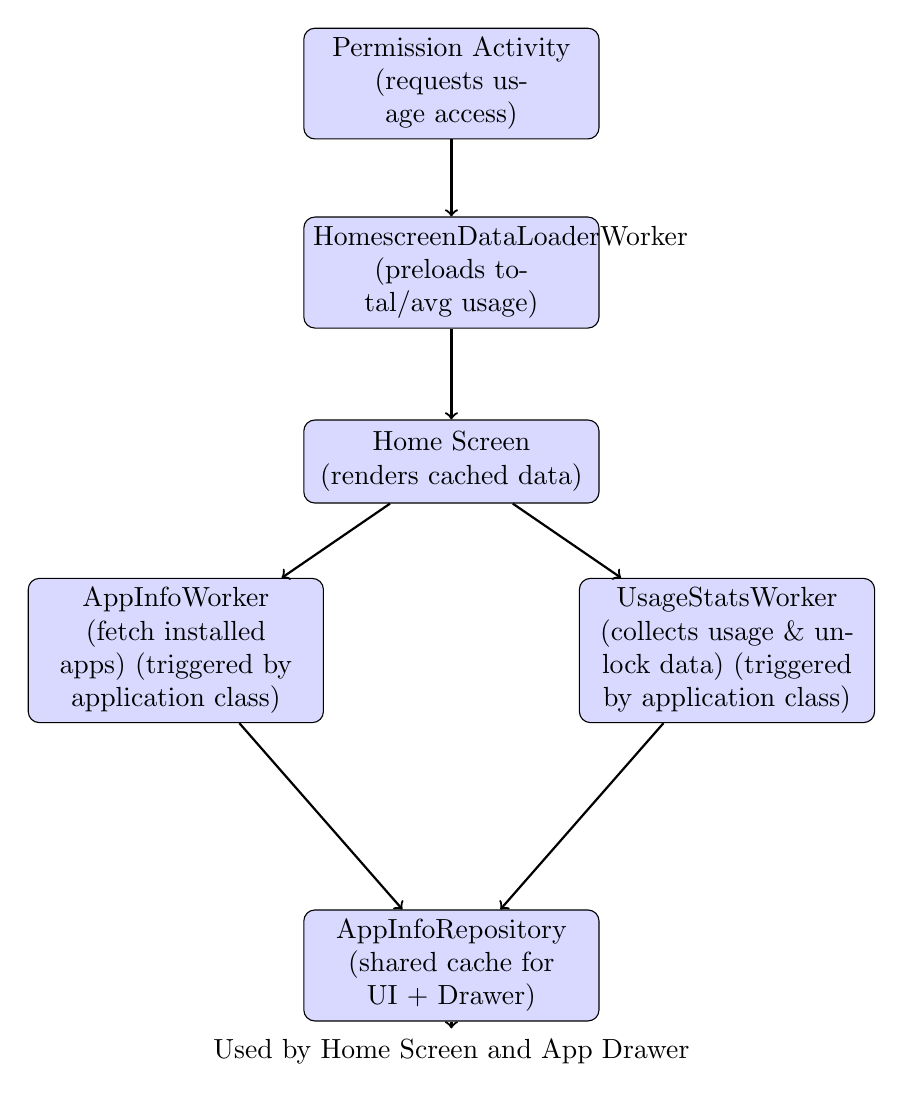
\begin{tikzpicture}[node distance=2.4cm, auto]
        % Nodes
        \node (perm) [block] {Permission Activity \\ (requests usage access)};
        \node (homeLoader) [block, below of=perm] {HomescreenDataLoaderWorker \\ (preloads total/avg usage)};
        \node (home) [block, below of=homeLoader] {Home Screen  \\ (renders cached data)};
        \node (appInfo) [block, below of=home, xshift=-3.5cm] {AppInfoWorker \\ (fetch installed apps) (triggered by application class)};
        \node (usage) [block, below of=home, xshift=3.5cm] {UsageStatsWorker \\ (collects usage \& unlock data) (triggered by application class)};
        \node (repo) [block, below of=home, yshift=-4cm] {AppInfoRepository \\ (shared cache for UI + Drawer)};
    
        % Arrows
        \draw[arrow] (perm) -- (homeLoader);
        \draw[arrow] (homeLoader) -- (home);
        \draw[arrow] (home) -- (appInfo);
        \draw[arrow] (home) -- (usage);
        \draw[arrow] (appInfo) -- (repo);
        \draw[arrow] (usage) -- (repo);
        \draw[arrow] (repo) -- ++(0,-0.8) node[below]{Used by Home Screen and App Drawer};
    \end{tikzpicture}
    \end{center}
    \footnote{Comment addressed :Overall workflow diagram needed - what are the various worker threads? What does each worker thread do?}
    \section{Nov 10 2025 - Nov 16 2025}
    {\bf No. of Hours: 5}
    \subsection{List of task completed:}
    \begin{enumerate}
        \item Fixed bug: Pressing home button from app drawer should open the home screen b
        \item Fixed bug: App drawer was getting empty on comming back to the drawer after some time.
        \item Fixed bug: app drawer was not refreshing on app install and uninstall
     \section{Nov 17, 2025 -- Nov 23, 2025}
    \textbf{No. of Hours: 10}
    
    \begin{enumerate}
        \item Refactored the app data layer to persist \textbf{installed apps, usage data, and home-screen statistics} in the Room database instead of in-memory structures. This enables reliable state restoration, especially during device reboots.
        
        \item Updated \textbf{AppInfoRepository} to:
        \begin{itemize}
            \item Store and serve a merged list of installed apps with usage data directly from the database.
            \item Provide \texttt{LiveData<List<AppWithUsage>>} and \texttt{LiveData<UsageSummaryEntity>} to consumers.
        \end{itemize}
    
        \item Refactored \textbf{LauncherViewModel} to observe the new DB-backed LiveData sources and remove all previous manual recomputation logic.
    
        \item Updated \textbf{HomeScreenFragmentMinimal}:
        \begin{itemize}
            \item Replaced manual computation of today/7-day usage with real-time values fetched from the DB.
            \item Added full null-safe UI binding to avoid boot-time crashes when the DB is not yet initialized.
        \end{itemize}
    
        \item Refactored \textbf{AppsDrawerFragment} and \textbf{AppListAdapter}:
        \begin{itemize}
            \item Removed redundant in-memory icon caching.
            \item Icons are now loaded dynamically using the system \texttt{PackageManager}, ensuring consistency and reducing database/storage overhead.
        \end{itemize}
    
        \item Rewrote \textbf{PackageInstallUnInstallReceiver}:
        \begin{itemize}
            \item Updated to work with the new \texttt{AppWithUsage} model.
            \item Ensures correct DB updates (add/remove apps) and triggers LiveData refresh for the UI.
        \end{itemize}
    
        \item Updated \textbf{AppDao}, entities (\texttt{AppInfoEntity}, \texttt{AppUsageEntity}, \texttt{UsageSummaryEntity}), and \textbf{AppWithUsage} model to support persistent usage tracking and merged app information.
    
        \item Improved all background \textbf{WorkManager workers}:
        \begin{itemize}
            \item Ensured \texttt{AppInfoWorker}, \texttt{UsageStatsWorker}, and \texttt{HomescreenDataLoaderWorker} write results directly to the DB.
            \item Fixed initialization timing issues that caused crashes at device boot.
        \end{itemize}
    
        \item \textbf{Bug Fix:} Resolved a long-standing issue where daily and 7-day app usage statistics were not being calculated or persisted correctly. Usage computation is now accurate and fully synchronized with the DB.
    \end{enumerate}
    \subsection*{Benefits of This Week’s Refactoring}
    \begin{enumerate}
      
        \item \textbf{Improved Battery Efficiency:} Heavy app–usage computations were moved to background workers and persisted in the database, reducing repeated processing on every screen open and lowering CPU wakeups.
        \item \textbf{Faster UI Performance:} App Drawer and Home Screen now load instantly since data comes directly from the local database and icons are fetched efficiently through the \texttt{PackageManager}.
        \item \textbf{Higher Reliability:} Fixed boot-time crashes and removed race conditions by adopting a single source of truth (Room DB) for app info and usage stats.
        \item \textbf{Cleaner Architecture \& Maintainability:} Refactored ViewModel, Repository, Workers, and Receiver for consistency, removing redundant in-memory storage and reducing code complexity.
    \end{enumerate}
    \section{Dec 02 2025 to Dec 07 2025}
    {\bf Number of Hours: 10}
    \subsection{List of Task Completed:}
    \begin{enumerate}
        \item Fixed launcher app drawer was showing wrong usage data (usage time and launch count).
        \item Fixed: App was crashing on Device reboot.
        \item Added some logs in launcher to understand which life cycle method for activity and fragments are called when.
    \end{enumerate}
    
    \section{ Dec 09 2025 to Dec 14 2025}
    {\bf No. of Hours: 15}
    \begin{enumerate}
        \item Fixed bug to update app info and app usage entry in app database when a new app is installed or an existing app is uninstalled and auto refresh the app drawer.
        \item Fixed: Application not responding bug on Home Screen due to heavy computation for progress bar(emoji feedback), moved it to background thread to save computation on main thread(UI thread is only updating the UI).
        \item Instead of storing all the app icons in the app storage dynamically load the icon from phone storage using package manager to save the space occupied by the application.
    \end{enumerate}
    \section{Dec 15 2025 to Dec 21 2025}
    {\bf No. of Hours: 10}
    \begin{enumerate}
        \item Created poster for survey.
        \item Done survey In MoodI for 3 days.
        \item Got 58 responses in the survey. 
        \item Sent GitHub branch details and access to repo for deploying app at play store.
    \end{enumerate}
    \section{Dec 22 2025 to Dec 31 2025}
    {\bf No. of Hours : 10}
    \subsection{To Do:}
    \begin{enumerate}
        \item Focus on the Notification foreground service to reduce the battery consumption.
        \item Stop asking battery exemption permission.
        \item Survives Doze / App Standby
        \item Instead of continuous polling based approach event based approach can reduce the battery consumption by the foreground service.
        \item \textbf{Event driven logic: }
        \begin{enumerate}
            \item Unlock
            \item App Entry
            \item Overlay focus change
            \item Home/ recents
            \item Screen Off.
        \end{enumerate}
        \item \textbf{Full Flow: }
        \begin{enumerate}
            \item SCREEN\_ON
     
     \item ↓
     \item KEYGUARD\_LOCKED
    \item ↓
    \item Lock overlay
     \item ↓
    \item  USER\_PRESENT
    \item  ↓
    \item Delayed foreground check
     \item ↓
    \item Overlay shown
     \item ↓
    \item Overlay loses focus OR Home OR Call OR Screen off
    \item  ↓
    \item Overlay removed
     \item ↓
    \item Next app entry → repeat
    \end{enumerate}
    \item \textbf{Why this does NOT miss cases: }
    \begin{table}[h]
    \centering
    \caption{Coverage of User Interaction Scenarios by Event-Driven Overlay Logic}
    \label{tab:overlay-coverage}
    \begin{tabular}{|l|l|}
    \hline
    \textbf{Scenario} & \textbf{Covered By} \\ \hline
    App opened via launcher & USER\_PRESENT + UsageStats \\ \hline
    App opened via notification & USER\_PRESENT + UsageStats \\ \hline
    App switch mid-session & Overlay focus loss \\ \hline
    Same app reopened & Cooldown logic \\ \hline
    Rapid app switching & Home / focus loss \\ \hline
    Screen locked & SCREEN\_OFF \\ \hline
    Incoming call & PHONE\_STATE \\ \hline
    \end{tabular}
    \end{table}
    
    \subsection{List of Task Completed}
    \begin{enumerate}
        \item Stopped tracking foreground app and notification update when the device is locked and resume this proces when the device is unlocked to reduce the battery consumption made by the app. (Achieved using broadcast reciever for USER\_PRESENT and SCREEN\_OFF)
        \item Moved all the reciever to single folder.
        \item Stopped asking permission for battery optimization and disable app usage during on-boarding as we no longer need it we can restart the monitoring or service from the launcher if it killed by Android OS.
    \end{enumerate}
    \end{enumerate}
    \section{Jan 5 2026 to Jan 11 2026}
    {\bf No. of Hours : 20}
    \subsection{TO DO: }
    \begin{enumerate}
        \item Deploy application on play store.
        \item create data usage policy file (if needed). 
        \item Add logs in all the activities to see which feature is mostly used by users (for user study analysis).
        \item Use HTTPS instead of HTTP for data transfer between client and server.
    \end{enumerate}
    \subsection{Survey Summary and Key Observations}
    
    Table~\ref{tab:survey_summary} presents a high-level summary of the user survey conducted to understand smartphone and social media usage patterns, perceived importance of reducing screen time, and related behavioral indicators.
    
    \begin{table}[h]
    \centering
    \caption{Summary of Survey Responses on Smartphone and Social Media Usage}
    \label{tab:survey_summary}
    \begin{tabular}{|p{5cm}|p{8cm}|}
    \hline
    \textbf{Aspect} & \textbf{Summary of Observations} \\
    \hline
    Total Participants & Total 58 respondents \\
    \hline
    Age Group Distribution & Majority of participants belong to the 18--22 age group, followed by 23--26; very few under 18 and above 27 \\
    \hline
    Gender Distribution & Predominantly male respondents, with a significant number of female participants \\
    \hline
    Family Income Range & Diverse economic backgrounds; most respondents fall below rupees 5 lakhs annual family income \\
    \hline
    Daily Social Media Usage & Wide variation observed, ranging from 1--2 hours to more than 10 hours per day; a large fraction reports 4--8 hours daily usage \\
    \hline
    Importance of Reducing Screen Time & High overall concern: most respondents rated importance as 4 or 5 on a 5-point scale \\
    \hline
    Most Used Applications & Instagram, WhatsApp, and YouTube dominate usage across respondents; Snapchat, Telegram, Reddit, and Twitter/X appear less frequently \\
    \hline
    Daily Device Unlock Frequency & Majority of users unlock their phones 50--150+ times per day, indicating habitual checking behavior \\
    \hline
    Discomfort with Idleness & Many respondents report discomfort when doing nothing, suggesting a tendency toward constant digital engagement \\
    \hline
    Actual Phone Usage (Digital Well-being) & Self-reported actual usage often aligns with or exceeds perceived usage, commonly falling between 5--8 hours per day \\
    \hline
    \end{tabular}
    \end{table}
    \subsection{Battery optimization changes: }
    \begin{enumerate}
    \item Stopped querying usage stats every minute from foreground service thread (for showing usage data on home screen, lock screen, and notification screen)
    \item Instead of querying usage stats every time use: Prefix sum approach store the already queried usage in shared pref and time stamp for last query and add the newly generated usage stats from last queried time to current query time.
    \item Every time home screen onResume function is called just calculate the time diff between the last time when the home screen was stopped and time now, this will be foreground time for all the apps other than launcher.
    \item For unlock count instead of querying unlocks every minute do use USER\_PRESENT Broadcast and increment the unlock count value saved in shared pref.
    \item Added periodic worker to reset usages shown in the app drawer at 5PM every-day.
    \subsection{Upload log file to the server for user study analysis: }
    \item Added models and API to upload file to server for user study analysis part.
    \item Added Android side changes to upload log file to server every 12 hours and clear the log file once upload is successful.
    \end{enumerate}
    \section{Feb 23 2026 to Mar 01 2026}
    {\bf No. of Hours: 5}
    \subsection{List of Task Completed}
    \begin{enumerate}
        \item Read libraries code available online for solving usage stats related bugs.
        \item Read How other launchers handle HomeScreen and AppDrawer.
    \end{enumerate}
    \subsection{To Do}
    \begin{enumerate}
        \item Focus on making the app more stable.
        \item Test every feature thoroughly and try to come up with possible fixes.
        \item Correct the phone usage,unlock count and app usage count calculation logic.
        \item Use android usestate API functions do not calculate usage in the app.
        % \item Customize timer settings to have multiple timer durations.
        \item Learn about firebase and it's setup.
        \item Remove exact alarm permission and use firebase instead.
        \item Change the permission flow don't ask to much permission on on-boarding as user as generally scared to grant so many permission in the beginning.
        \item Fix graph layout: Make it a proper dashboard like famous apps like: Digital well-Being, StayFree or use secure Digital wellbeing APIs from our App if any .
    \end{enumerate}
    \section{Feb 23 2026 (last meeting) to Mar 05 2026}
    {\bf No. of Hours: 16}
    \subsection{List of Task Completed}
    \begin{enumerate}
        \item Fixed unlock count API returning inconsistent value of Unlock count.
        \begin{enumerate}
            \item \textbf{Earlier Logic: } Count \# of \textbf{KEYGAURD\_SHOWN} event in the passed interval, it was also counting some key gaurd shown events in which user have not unlocked the phone but just pressed the power button and this event got triggered.
            \item \textbf{Current Logic: } Count \# of \textbf{KEYGAURD\_HIDDEN} event, counting this event can give accurate result as \textbf{KEYGAURD\_HIDDEN} event is fired after the user is done with unlocking and key gaurd is about to disappear.
            \item Fixed: JoDo App was crashing when the Device boots up, because on boot the whole app process is recreated by android.
            \begin{enumerate}
                \item \textbf{Earlier: } Load data from Room Database which is stored in Hard Disk .
                \item \textbf{Now: } Created two shared prefs(Act as cache),which are very light weight and reading them will take less time as compared to quering the DB entries. Though shared prefs persist data across process lifecycle, it is saved in Hard-disk it is loaded in main memory during runtime which makes it to access faster as compared to room db.
                 \end{enumerate}
                \item \textbf{Room DB and SharePrefs Cache: } On every background worker run, data is saved in Room db and copied to SharedPref cache, and when UI observe the Live data, Repository can get data from either cache or DB.
                \item The above process follows the \textbf{MVVM} architecture: \textbf{Model} \textbf{View} \textbf{ViewModel}, and with the help of view model UI state can be reused,survive config changes and process restart after being killed by Android OS.
                \item With the help of the the Repository we can have multiple data storage and Repo can give which ever data is available to ViewModel and from ViewModel to View(UI), in this UI can be loaded fast on process restart.
                \item \textbf{Fixed Bug: } Home screen Was crashing Due to \textbf{Integer Overflow} as usage time value in Millisecond can be very high and can cross Integer limit and result in App Crash (From progress bar logic Home-screen)
                \item Studied about Firebase and it's integration in Android Application.
                \item Found out that Firebase is also not very time bound, it has almost similar delay as WorkManager.
                \item As JoDo app is currently got accepted by play store( \href{https://play.google.com/store/apps/details?id=in.ac.iitb.cse.jodo&pcampaignid=web_share}{link}),  so I am not planing to integrate Firebase as Exact alarm is working fine and on time.
               
                
           
        \end{enumerate}
    \end{enumerate}
    \subsection{To Do}
    \begin{enumerate}
        \item Change permission flow as user are getting scared because of \# of permissions are too much (Pilot study feedback)
        \item Do not ask so much permission in the beginning.
        \item Delay the \textbf{Default Home Screen permission} to later, after the user come back to the app ask home screen permission, because \textbf{Home Screen} is something which changes the whole mobile phone interaction interface, asking in the begining may result in user loss.
        \item Delay the Pause App Activity permission to atleast one day after Installation.
        \item In the begining only ask : \textbf{Usage stats, overlay on app, Battery optimization and Notification} permission.
        \item Make Lock screen optional, ask user a permission to act as LockScreen.
         \item Add Age Restriction of above 16 or 18 (will decide according to current standards).
         \item Give Drop Down for gender selection.
    \end{enumerate}
    \end{enumerate}
    \section{Mar 06 2026 (last meeting) to Mar 10 2026}
    {\bf No. of Hours: 16}
    \subsection{List of Task Completed}
    \begin{enumerate}
        \item Changed permission flow: removed \textbf{Default launcher}, \textbf{Pause App Activity when unused} during on-boarding.
        \item Made \textbf{Read call logs} permission optional.
        \item Instead of single screen, created five layout files and reused same fragment to ask permission for on every screen.
        \item Used viewpager adapter to switch between Permission Fragments.
        \item Added drop down to ask gender.
        \item Added age limit above 13 year.
        \item Added a small setting icon on home screen, after atleast 7 day of installation we can ask pause app activity permission (To Do).
    
        \item Added permission to make JoDo as Lock screen, stored it in the shared prefs, and shown lock screen accordingly.
        \item Changed background of all the onboarding screen to black including login and register screen 
        
    \end{enumerate}
    \subsection{New vs Old UI comparision}
    \begin{figure}[H]
        \centering
        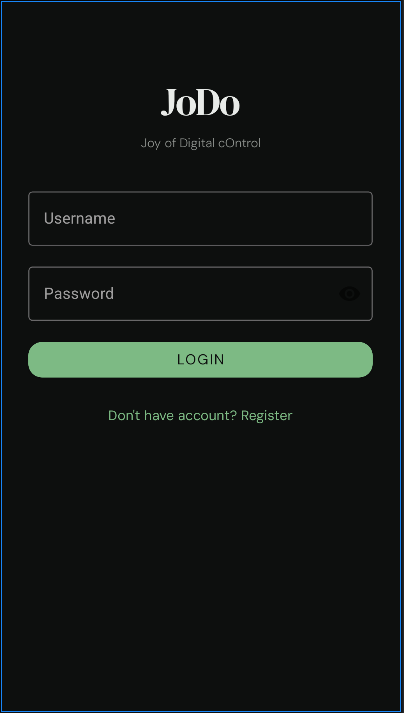
\includegraphics[width=0.50\linewidth,height=0.50\textheight, keepaspectratio]{login-screen-new.png}
        \hspace{0,3cm}
        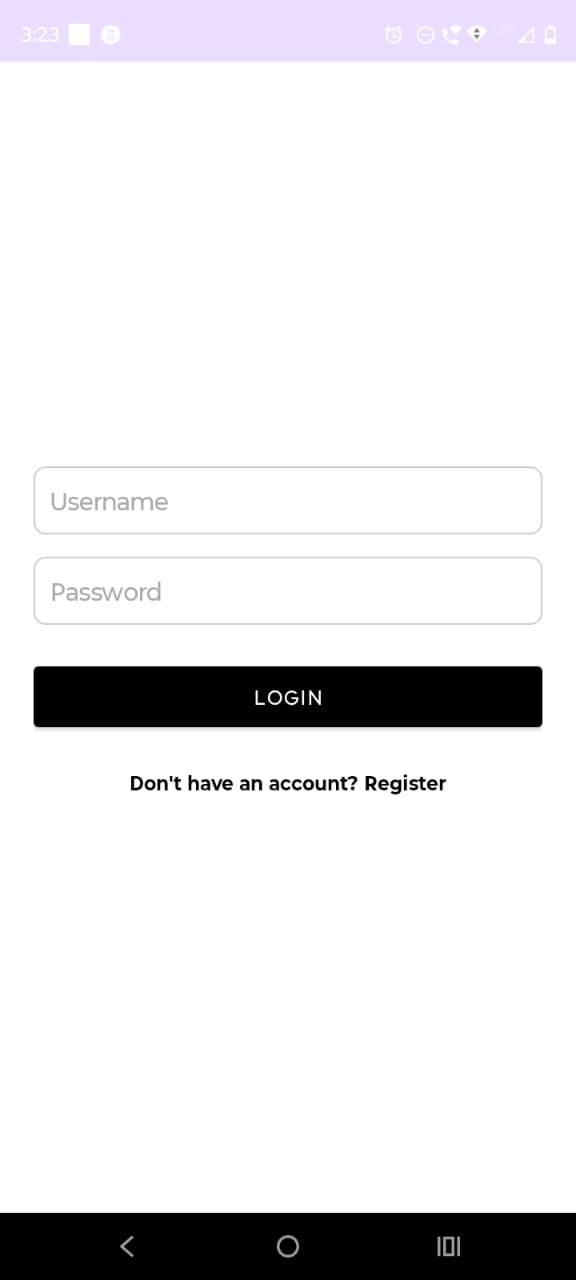
\includegraphics[width=0.50\linewidth, height=0.50\textheight, keepaspectratio]{login-screen.jpeg}
    
         \vspace{0.5cm}
    
        % 
\includegraphics[width=0.45\linewidth]{JoDo new UI design/dashboard.png}
        % 
\includegraphics[width=0.45\linewidth]{JoDo new UI design/lock_screen.png}
    
        \caption{Login-screen-new(left),Login-screen-old(right)}
        \label{fig:ui_prototype}
    \end{figure}
    \begin{figure}[H]
        \centering
        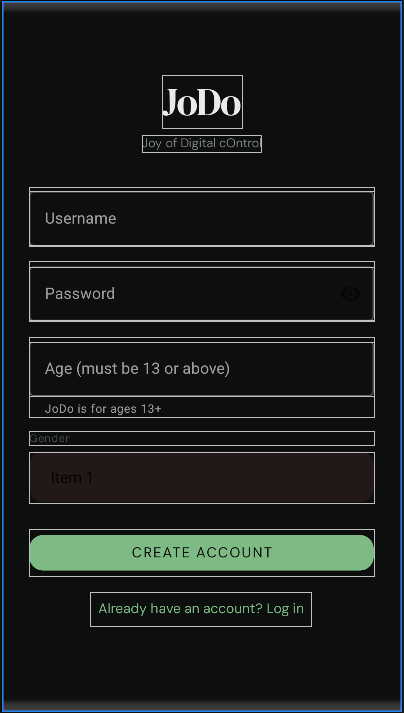
\includegraphics[width=0.50\linewidth,height=0.50\textheight, keepaspectratio]{register-scree-new.png}
        \hspace{0,3cm}
        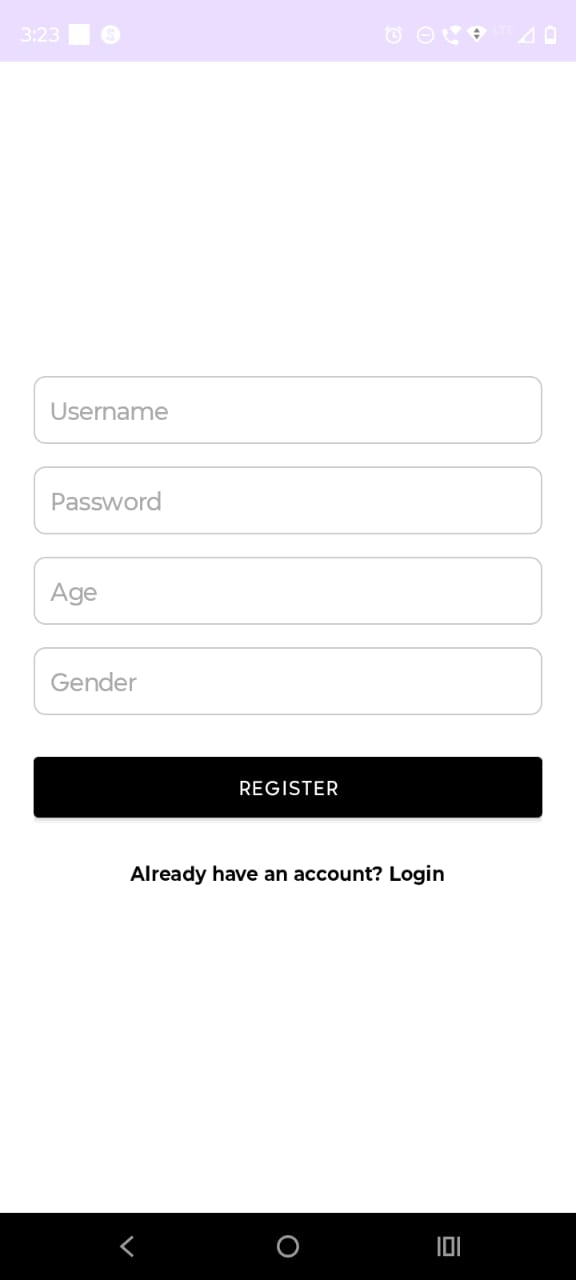
\includegraphics[width=0.50\linewidth, height=0.50\textheight, keepaspectratio]{register-screen.jpeg}
    
         \vspace{0.5cm}
    
        % 
\includegraphics[width=0.45\linewidth]{JoDo new UI design/dashboard.png}
        % 
\includegraphics[width=0.45\linewidth]{JoDo new UI design/lock_screen.png}
    
        \caption{Register-screen-new(left),Register-screen-old(right)}
        \label{fig:ui_prototype2}
    \end{figure}
    \begin{figure}[H]
        \centering
        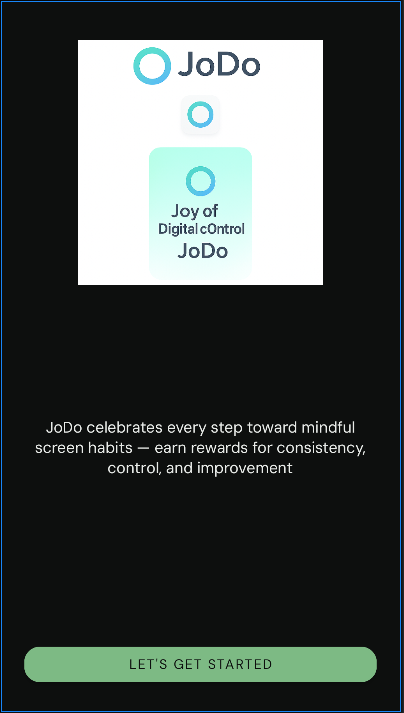
\includegraphics[width=0.50\linewidth,height=0.50\textheight, keepaspectratio]{onboarding-screen-new.png}
        \hspace{0,3cm}
        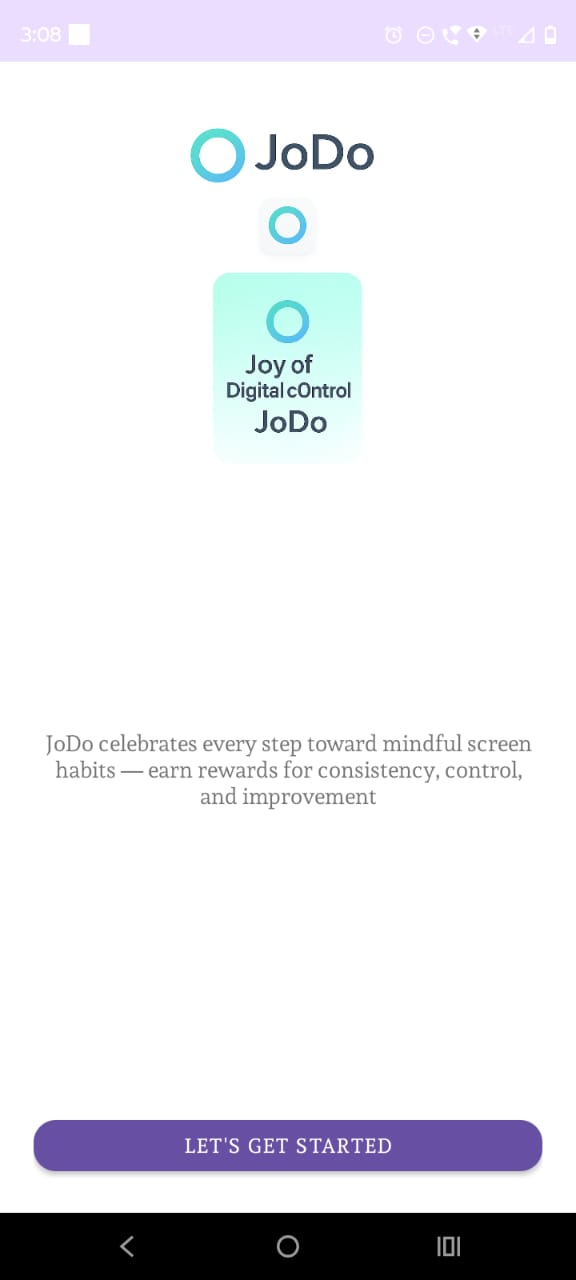
\includegraphics[width=0.50\linewidth, height=0.50\textheight, keepaspectratio]{get-started-screen.jpeg}
    
         \vspace{0.5cm}
    
        % 
\includegraphics[width=0.45\linewidth]{JoDo new UI design/dashboard.png}
        % 
\includegraphics[width=0.45\linewidth]{JoDo new UI design/lock_screen.png}
    
        \caption{GetStarted-screen-new(left),GetStarted-screen-old(right)}
        \label{fig:ui_prototype3}
    \end{figure}
    
    \begin{figure}[H]
        \centering
        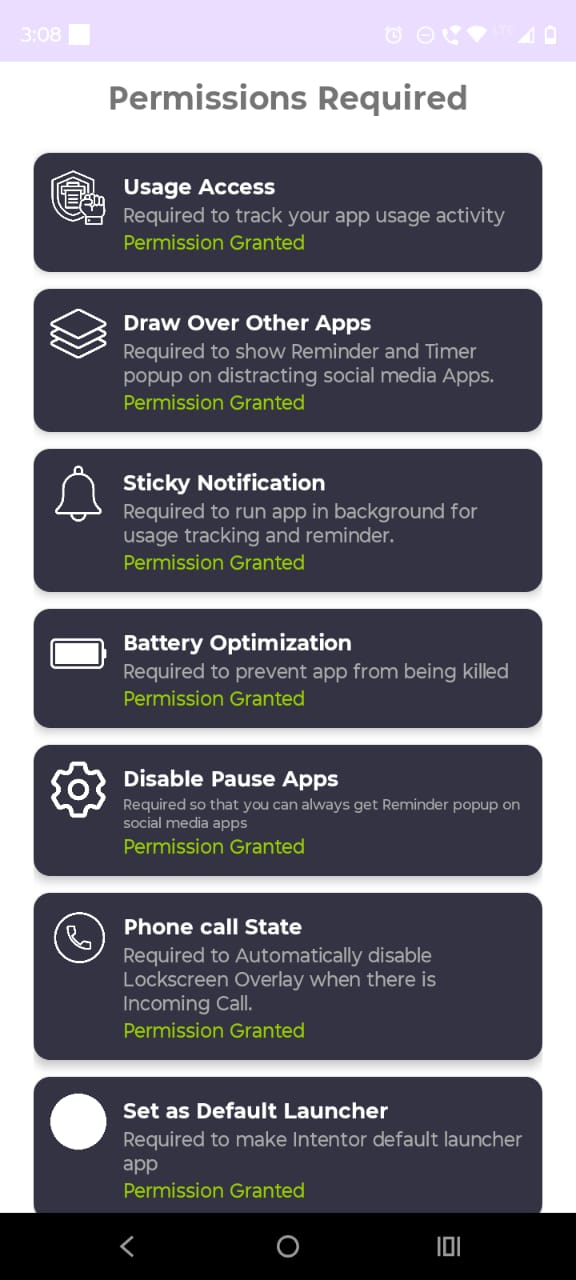
\includegraphics[width=0.50\linewidth,height=0.50\textheight, keepaspectratio]{permission-screen.jpeg}
        \hspace{0,3cm}
        % 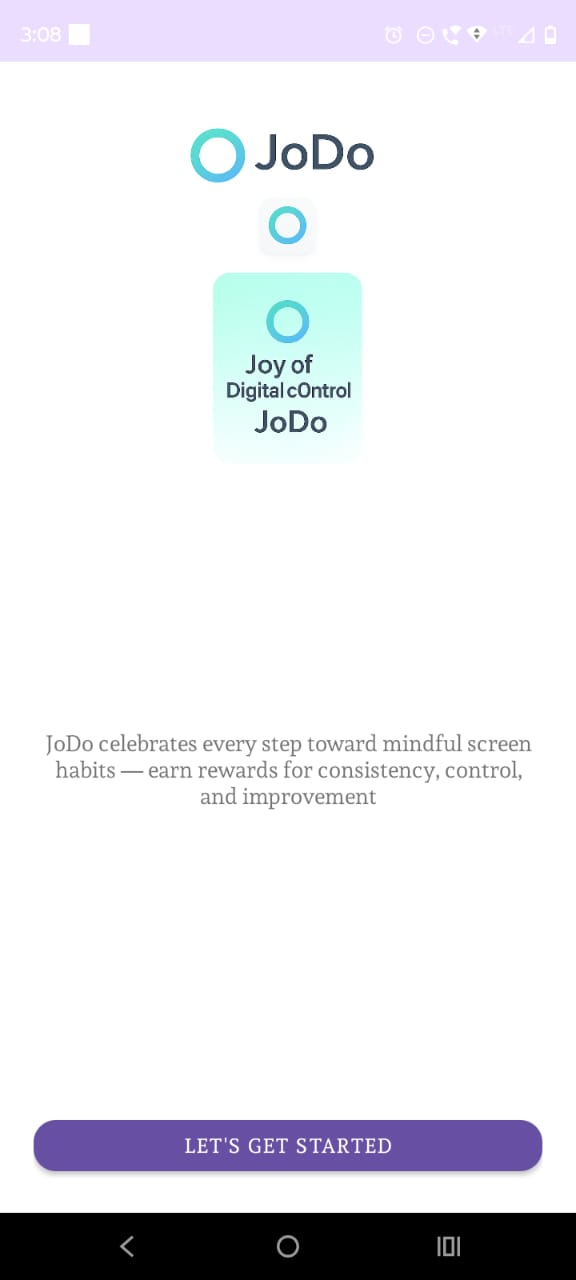
\includegraphics[width=0.50\linewidth, height=0.50\textheight, keepaspectratio]{get-started-screen.jpeg}
    
         \vspace{0.5cm}
    
        % 
\includegraphics[width=0.45\linewidth]{JoDo new UI design/dashboard.png}
        % 
\includegraphics[width=0.45\linewidth]{JoDo new UI design/lock_screen.png}
    
        \caption{Permission-screen-old}
        \label{fig:ui_prototype4}
    \end{figure}
    \begin{figure}[H]
        \centering
        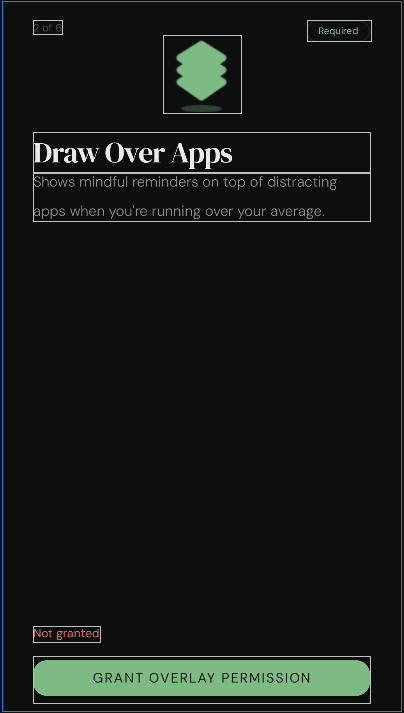
\includegraphics[width=0.50\linewidth,height=0.50\textheight, keepaspectratio]{draw-over-app-permission.png}
        \hspace{0,3cm}
        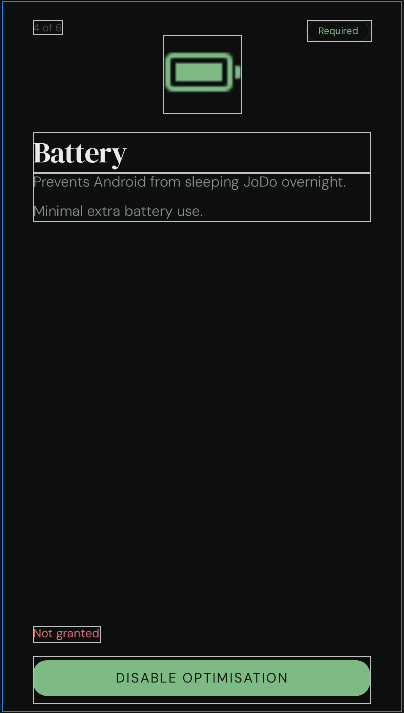
\includegraphics[width=0.50\linewidth, height=0.50\textheight, keepaspectratio]{battery-optimization-permission.png}
    
         \vspace{0.5cm}
    
        % 
\includegraphics[width=0.45\linewidth]{JoDo new UI design/dashboard.png}
        % 
\includegraphics[width=0.45\linewidth]{JoDo new UI design/lock_screen.png}
    
        \caption{New Permission UI}
        \label{fig:ui_prototype5}
    \end{figure}
    \begin{figure}[H]
        \centering
        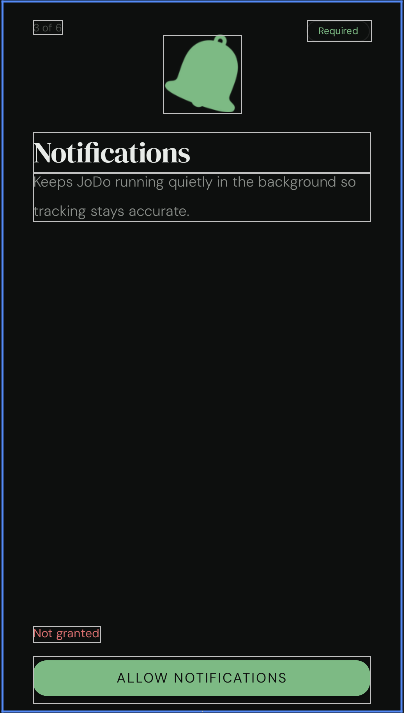
\includegraphics[width=0.50\linewidth,height=0.50\textheight, keepaspectratio]{notification-permission.png}
        \hspace{0,3cm}
        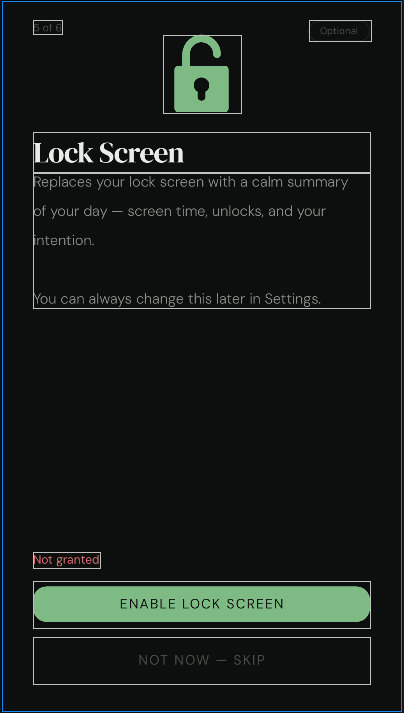
\includegraphics[width=0.50\linewidth, height=0.50\textheight, keepaspectratio]{lock-screen-permision.png}
    
         \vspace{0.5cm}
    
        % 
\includegraphics[width=0.45\linewidth]{JoDo new UI design/dashboard.png}
        % 
\includegraphics[width=0.45\linewidth]{JoDo new UI design/lock_screen.png}
    
        \caption{New Permission UI}
        \label{fig:ui_prototype6}
    \end{figure}
    \begin{figure}[H]
        \centering
        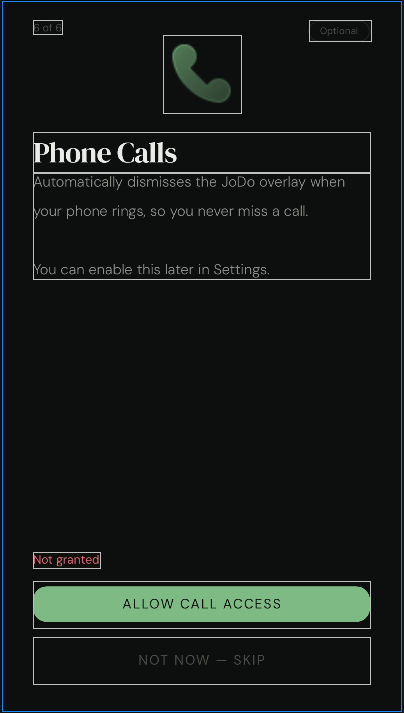
\includegraphics[width=0.50\linewidth,height=0.50\textheight, keepaspectratio]{phone call permission.png}
        \hspace{0,3cm}
        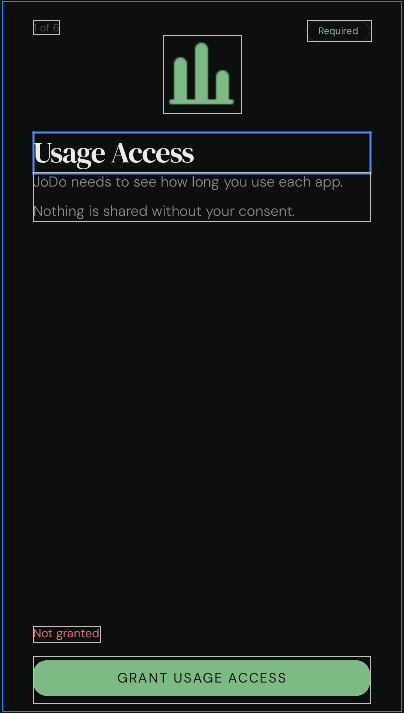
\includegraphics[width=0.50\linewidth, height=0.50\textheight, keepaspectratio]{usage-states-permission.png}
    
         \vspace{0.5cm}
    
        % 
\includegraphics[width=0.45\linewidth]{JoDo new UI design/dashboard.png}
        % 
\includegraphics[width=0.45\linewidth]{JoDo new UI design/lock_screen.png}
    
        \caption{New Permission UI}
        \label{fig:ui_prototype7}
    \end{figure}
    \section{Mar 11 2026 (last meeting) to Mar 12 2026}
    {\bf No. of Hours: 10}
    \subsection{List of Task Completed}
    \begin{enumerate}
         \item Studied Nginx as a reverse proxy, API gateway, load balancer and it's benefits.
         \item We can intergrate reverse proxy, API gateway, load balancer,internal DDos protection in single Nginx instance.
         \item Created Nginx config file.
        \item Installed Nginx in docker container at server.
         \item Added Nginx as an reverse proxy or API gateway, for all the APIs applied global rate limit of 50 request per day.
        \item Nginx will forward all the trafic coming at port 80 to the django docker container at port 8000.
        \item Earlier we were exposing port 8000 to now Nginx can hide it.
        \item Added directive (Key value config) for different context (parts of whole config) like events, server,location, etc. 
        \item Added rate limit config in Nginx.
         \item Used Django Axes to protect from brute force attack where user can change ip but Axes track combination of IP and username as we don't have username info at nginx server.
         \item Disabled port 8000 using ufw firewall.
         \item Removed port from the API as default port 80 will be used for http communication.
         \item set up Nginx as a cache as well, and served static files directly from nginx.
         \item To serve staticfiles, nginx share volume with Django app.
    \end{enumerate}
    \subsection{To Do}
    \begin{enumerate}
        \item Change UI background color, make every screen background black.
        \item Modify the DashBoard to Look like modern Dashboard.
        \item Combine : \textbf{Points,Usage,unlocks,App launches } history in a single dashboard.
        \item Modify the reward reveal animation, make it feel like real basketball hit.
        \item Create the Rounded Corner logo for JoDo App.
    \end{enumerate}
 \section{Mar 13 2026 (last meeting) to Mar 17 2026}
{\bf No. of Hours: 10}
\subsection{Task Completed}
\begin{enumerate}
    \item Added API in app repository to reset usage data in db at 5pm so that app drawer does not show previous day data after 5pm.
    \item Made foreground service of type special, earlier it was of type data sync, latest android version limits total foreground time for datasync services to 6 hours.
    \item Created Retrofit API to upload log file every day to the server.
    \item Create a periodic worker to upload log every 24 hours and scheduled it from Application class.
\end{enumerate}
\subsection{To Do}
\begin{enumerate}
    \item Test the newly added code on different Android devices
\end{enumerate}
\section{Mar 18 2026 to Mar 23 2026}
{\bf No. of Hours: 5}
\subsection{Work Done}
\begin{enumerate}
    \item Added config in nginx.conf to add Nginx as reverse proxy for his backend application.
    \item Added shared docker network used by both Nginx and gaurav's web application.
    \
\end{enumerate}
\end{document}
    